\documentclass[11pt,a4paper]{article}
\usepackage[margin=2.4cm]{geometry}
\usepackage{amsmath,amssymb,bm}
\usepackage{graphicx}
\usepackage{booktabs}
\usepackage{siunitx}
\usepackage[table]{xcolor}
\usepackage{caption}
\usepackage{longtable}
\usepackage[colorlinks=true,linkcolor=blue!55!black,citecolor=blue!55!black,
            urlcolor=blue!55!black]{hyperref}


\usepackage[protrusion=true,expansion=false]{microtype}

\sisetup{scientific-notation=true, round-mode=places, round-precision=1}
\newcommand{\Shat}{\bm{S}}
\newcommand{\eqBH}[1]{eq.~(#1)}
\newcommand{\code}[1]{\texttt{#1}}
\captionsetup{font=small,labelfont=bf}

\title{\bfseries Exact partial structure factors for polydisperse\\
hard-sphere--Yukawa and sticky-hard-sphere fluids,\\
with an assessment of the approximations used in SASfit}
\author{Prepared for J.\ Kohlbrecher, Paul Scherrer Institut (LNS)}
\date{\today}

\begin{document}
\maketitle

\begin{abstract}
\noindent
We report a complete, validated implementation of the analytic mean-spherical
approximation (MSA) solution for an $N$-component hard-sphere--Yukawa fluid,
following Blum \& Hernando [J.~Phys.: Condens.\ Matter \textbf{14}, 11933
(2002)], together with the resulting exact partial structure factors
$S_{ij}(Q)$ and a small-angle-scattering layer that maps a continuous size
distribution onto the model and produces the exact scattered intensity.
Establishing the implementation required correcting \emph{three} misprinted
equations and recognising \emph{one} systematic reading trap; a fourth printed
equation is internally inconsistent but is never needed. All three misprints
are invisible for a single component with a common coupling, and therefore
silently corrupt every polydisperse calculation while leaving every
single-component test passing. Each correction is derived from other equations
of the same paper rather than fitted, and the final result is verified against
three independent references: SASfit's compiled one-Yukawa library at $N=1$
(agreement to $\sim\!10^{-14}$ in the contact value and $\sim\!10^{-10}$ in
$S(Q)$), the exact Percus--Yevick hard-sphere and Lebowitz mixture limits as
$K\to0$, and a purpose-written numerical Ornstein--Zernike solver at $N>1$ that
shares no equation with the analytic route.

We then asked whether these corrections were already known, and found that two
of the three are: Blum's own later paper with Arias
[arXiv:cond-mat/0602477 (2006)] prints both of them in corrected form, with no
erratum, no footnote and no remark that anything had changed. Our corrections,
obtained by probing the paper's own recursion rather than by transcribing
anything, agree with that later paper to $10^{-15}$ while differing from the
2002 text by up to $18\%$. The third correction is likewise a silent fix in the
same 2006 paper. This is a cautionary result rather than a reassuring one: the
corrected equations exist in the literature, but only for a reader who thinks
to distrust the 2002 paper and to consult a preprint four years later that
never says why it differs. The sequel in turn carries a misprint of its own,
which our numerics locate.

The last of those corrections --- a single index in the definition of
$D_{ij}$ --- also removes what had appeared to be the main obstacle to
extending the theory: with it, charge (coupling) polydispersity
$\delta_i\neq1$ closes in \emph{closed form} rather than requiring a separate
derivation, and polydisperse RMSA, which maps onto exactly that case, becomes
analytic. We implement RMSA with a common rescaling factor chosen so that all
contact values are non-negative, and verify it against the independent
numerical solver to $0.006\%$ in the rescaling factor.

With an exact $S_{ij}$ available, we then quantify --- for the first time, as
far as we are aware --- the error of all six approximate schemes that SASfit
offers for combining a structure factor with a size distribution. Two results
are of practical consequence. First, the ``partial structure factor'' option is
statistically indistinguishable from the decoupling approximation in every case
tested, so the double integral it requires buys nothing. Second, the ranking of
the remaining schemes is \emph{not} universal: the local monodisperse
approximation is the best choice for repulsive interactions, but for attractive
ones the scaling approximation of Gazzillo \emph{et al.} is better by roughly a
factor of four. The common rule of thumb favouring the local monodisperse
approximation is therefore only half right.
\end{abstract}

\tableofcontents

\section{Introduction and scope}

Small-angle scattering from a concentrated dispersion measures the product of
particle form and inter-particle structure. For a \emph{monodisperse} system
this factorises cleanly into $P(Q)$ and $S(Q)$. For a polydisperse system it
does not: different size classes have different form factors \emph{and}
different mutual correlations, and the intensity becomes a double sum over
partial structure factors,
\begin{equation}
  I(Q)=\sum_{ij}\sqrt{n_i n_j}\,F_i(Q)F_j(Q)\,S^{\mathrm{AL}}_{ij}(Q),
  \label{eq:Iexact}
\end{equation}
with $S^{\mathrm{AL}}_{ij}=\delta_{ij}+\sqrt{n_in_j}\,\tilde h_{ij}(Q)$ the
Ashcroft--Langreth partials and $n_i$ the number density of class $i$.

Because $S_{ij}$ has rarely been available in closed form for a realistic
interaction, scattering analysis has relied on approximations that collapse
\eqref{eq:Iexact} back into something factorisable. SASfit implements six of
them. This report removes the need for that approximation in the
hard-sphere--Yukawa case, and then uses the exact result to measure how much
each approximation costs.

\paragraph{Scope and restrictions.} Throughout, the Yukawa coupling is
\emph{factored} with $\delta_i=1$: a single screening length and a common
contact strength shared by all species, with arbitrary polydispersity in
\emph{size}. Charge (coupling) polydispersity, $\delta_i\neq1$, is not covered
--- see \S\ref{sec:open}. The number of Yukawa terms is $M=1$ throughout. The
sticky-hard-sphere comparison uses SASfit's own Robertus engine, which likewise
takes the stickiness $\tau$ to be size-independent.

\paragraph{Provenance.} Per the repository's \code{AI\_USAGE.md}, the
derivations in \S\ref{sec:errata} were prepared as scaffolding and have been
independently verified by the author before being relied upon; this is stated
per item in that section. Every number quoted in this report is regenerated by
\code{report\_numbers.py} rather than transcribed.

\section{Theoretical background}

\subsection{Model and closure}

We take $N$ species with hard-core diameters $\sigma_i$ and number densities
$\rho_i$, interacting through a hard core plus a single Yukawa tail. Outside
contact the MSA closure fixes the direct correlation function
(Blum \& Hernando, hereafter BH02, \eqBH{5}),
\begin{equation}
  c_{ij}(r)=\frac{K_{ij}\,e^{-z(r-\sigma_{ij})}}{r},\qquad r>\sigma_{ij}
  =\tfrac12(\sigma_i+\sigma_j),
  \label{eq:closure}
\end{equation}
while the hard core fixes the pair correlation inside it,
$h_{ij}(r)=-1$ for $r\le\sigma_{ij}$ (\eqBH{6}). In the factored case
$K_{ij}=K\delta_i\delta_j$; with $\delta_i=1$ this is simply $K_{ij}=K$.
Because the MSA sets $c=-\beta U$ outside the core, the sign convention is the
opposite of what the form of \eqref{eq:closure} might suggest: a screened-Coulomb
\emph{repulsion} has $U>0$ and therefore $K<0$, while $K>0$ describes an
\emph{attraction}. This is confirmed by both independent indicators --- at
$\varphi=0.1$, $K=+1$ gives $g(\sigma^+)=2.13$ and $S(0)=0.636$, against the
hard-sphere values $1.296$ and $0.456$ (contact enhanced, compressibility
raised: attraction), while $K=-1$ gives $0.504$ and $0.348$ (contact depleted,
compressibility lowered: repulsion).

\subsection{Baxter--Wertheim factorisation}

The Ornstein--Zernike equation is solved by the Baxter--Wertheim
factorisation (BH02 \eqBH{7}, \eqBH{12}), which writes
$\bm I-\rho\tilde{\bm C}(k)$ as a product of a matrix analytic in the upper
half $k$-plane and its conjugate. The factor function $q_{ij}(r)$ has the
piecewise form (BH02 \eqBH{17},\eqBH{18})
\begin{align}
  q_{ij}(r)&=q^0_{ij}(r)+D^{(1)}_{ij}e^{-zr},\qquad \lambda_{ji}<r,\\
  q^0_{ij}(r)&=\tfrac12A_j\big[(r-\tfrac{\sigma_j}{2})^2-(\tfrac{\sigma_i}{2})^2\big]
   +\beta_j\big[(r-\tfrac{\sigma_j}{2})-\tfrac{\sigma_i}{2}\big]\nonumber\\
   &\quad+C^{(1)}_{ij}e^{-z\sigma_j/2}\big[e^{-z(r-\sigma_j/2)}-e^{-z\sigma_i/2}\big],
   \qquad \lambda_{ji}<r<\sigma_{ij},
\end{align}
with $\lambda_{ji}=\tfrac12(\sigma_j-\sigma_i)$. The unknowns are the Baxter
amplitudes $a_j$ and the auxiliary quantities $A_j$, $\beta_j$,
$C_{ij}$, $D_{ij}$ and $\hat B_j$.

\subsection{The Blum--Hernando solution}

The purely geometric quantities are
\begin{equation}
  \zeta_k=\sum_i\rho_i\sigma_i^k,\quad \Delta=1-\tfrac{\pi}{6}\zeta_3,\quad
  A^0_j=\frac{2\pi}{\Delta}\Big[1+\tfrac12\zeta_2\tfrac{\pi}{\Delta}\sigma_j\Big],
  \quad \beta^0_j=\frac{\pi}{\Delta}\sigma_j,
\end{equation}
and the solution is built from them by (BH02 \eqBH{23},\eqBH{24})
\begin{equation}
  A_j=A^0_j+\frac{\pi}{\Delta}a_jP,\qquad \beta_j=\beta^0_j+a_j\Delta^{(1)}.
\end{equation}
Three auxiliary functions recur throughout,
\begin{equation}
  \phi_0(x)=\frac{1-e^{-x}}{x},\quad
  \phi_1(x)=\frac{1-x-e^{-x}}{x^2},\quad
  \psi_1(x)=\frac{1-\tfrac{x}{2}-(1+\tfrac{x}{2})e^{-x}}{x^3},
  \label{eq:phipsi}
\end{equation}
all entire, and satisfying $\phi_1=x\psi_1-\phi_0/2$ (BH02 \eqBH{45}).

Two further vectors, $\Pi_j$ and $X_j$, carry the dependence on $\hat B$. BH02
gives them twice: once through matrices $\hat{\mathcal I},\hat{\mathcal J}$
(\eqBH{34}--\eqBH{39}), and once explicitly (\eqBH{30},\eqBH{32},\eqBH{33}),
\begin{align}
  \Delta^{(1)}&=-\frac{2\pi}{z^2\Delta}\sum_\ell\rho_\ell
     \Big(1+\tfrac{z\sigma_\ell}{2}\Big)\delta_\ell
     -\frac{2\pi}{\Delta}\sum_\ell\rho_\ell\sigma_\ell^3\psi_1(z\sigma_\ell)\hat B_\ell,
     \label{eq:BH30}\\
  X_i&=\delta_i+\sigma_i\phi_0(z\sigma_i)\hat B_i+\sigma_i\Delta^{(1)},
     \label{eq:BH33}\\
  \Pi_j&=\hat B_j+\Big(1+\tfrac{\sigma_jz}{2}\Big)\Delta^{(1)}
     +\tfrac{\sigma_j}{2}\sum_\ell\rho_\ell\beta^0_\ell X_\ell.
     \label{eq:BH32}
\end{align}
That redundancy is what makes the errata of \S\ref{sec:errata} detectable.

\subsection{Closing the system}

Two equivalent routes close the problem. The first solves the primary MSA
closure (BH02 \eqBH{55}) for the $N$ amplitudes $a_j$, with $\hat B$ obtained
from its own linear self-consistency (\eqBH{62}--\eqBH{64}). The second uses
the scaling structure of \S4 of BH02: \eqBH{72} states
$\Pi_i=-\Gamma X_i$ with $\Gamma$ a scalar at $M=1$, which is linear in
$\hat B$ at fixed $\Gamma$, and \eqBH{100b},
\begin{equation}
  2\pi K=-\frac{2\Gamma(z+\Gamma)}{D_2},\qquad D_2=\sum_k\rho_kX_k^2,
  \label{eq:gammaclosure}
\end{equation}
supplies the one remaining scalar equation, with the amplitudes then
\emph{derived} as $a_j=2\Gamma X_j/D_2$. The whole problem reduces to a
one-dimensional root find in $\Gamma$.

Both are implemented (\code{solve()} and \code{solve\_gamma()}) and, once the
errata below are applied, they agree to machine precision. They are retained as
mutual cross-checks: they carry different unknowns, so agreement is
informative rather than tautological. The $\Gamma$ route additionally handles
$K=0$ exactly, where the other degenerates.

\section{Errata in the published equations}
\label{sec:errata}

Five separate obstacles had to be cleared before the implementation closed.
They are not all of the same kind, and it matters to keep them apart --- a
distinction earlier drafts of this report did not draw sharply enough.
\emph{Three} are genuine misprints: an equation as printed says something the
authors demonstrably did not mean, and the corrected form is forced by other
equations of the same paper. \emph{One} is an internal inconsistency in an
equation we do not need. And \emph{one} --- the one that cost the most time
--- is not an error in the paper at all, but a trap for the implementer: an
equation that is entirely correct for what it states, and that states something
other than what a reader building a structure-factor code is looking for.

The three misprints share a property that explains how they survived
peer review and twenty-four years of citation: each is invisible in the
simplest case. Two of them collapse to the correct expression whenever $N=1$,
because the two interchanged indices then take the same value; the third
collapses whenever all $\delta_i$ are equal, which is the case in every
application that does not model charge polydispersity. A single-component
validation against a reference implementation --- exactly the validation an
implementer would naturally run first, and exactly the one we ran --- passes at
machine precision with all three misprints still in place. This is worth
stating plainly because it undercuts a tempting inference: agreement with
published single-component numbers is \emph{not} evidence that the
multicomponent equations have been transcribed correctly.

Table~\ref{tab:errata} summarises the five items. Each correction is derived
below from \emph{other} equations of the same paper, never fitted to our
numerics; \S\ref{sec:literature} then asks, separately, whether each was
already known.

\begin{table}[htbp]
\centering
\small
\caption{The five items, classified. ``Simplest case'' indicates whether the
item has any effect on a single-component calculation with a common coupling
$\delta_i\equiv1$ --- that is, whether a monodisperse validation can see it.
The last column anticipates \S\ref{sec:literature}.}
\label{tab:errata}
\begin{tabular}{@{}lllll@{}}
\toprule
Equation & Kind & Nature & Visible in& Already in\\
         &      &        & simplest case & the literature?\\
\midrule
BH02 \eqBH{35} & misprint & $j\leftrightarrow\ell$ interchange & no &
  yes, BA \eqBH{76}\\
BH02 \eqBH{38} & misprint & $j\leftrightarrow\ell$ interchange & no &
  yes, BA \eqBH{76}\\
BH02 \eqBH{22} & misprint & $\delta$ on the column index & no &
  yes, BA \eqBH{25}\\
BH02 \eqBH{31} & inconsistent & disagrees with \eqBH{27}, \eqBH{28} & yes &
  not addressed\\
BH02 \eqBH{20} & \emph{correct} & is $q'$, not the contact value & --- &
  yes, BA \eqBH{26}\\
\bottomrule
\end{tabular}
\end{table}

\begin{table}[htbp]
\centering
\small
\caption{Cost of leaving each item uncorrected, measured on the three-component
test system of \S\ref{sec:external} ($\sigma=(1,1.5,2.5)$, $z=4$, $K=0.8$).}
\label{tab:erratacost}
\begin{tabular}{@{}ll@{}}
\toprule
Equation & Effect if uncorrected\\
\midrule
BH02 \eqBH{35} & $\sim2\times10^{-2}$ in $\Pi^{(n)}$; up to $18\%$ in
  $\hat{\mathcal I}$ at $z\sigma\sim2$\\
BH02 \eqBH{38} & $\sim10^{-2}$ in $X^{(n)}$\\
BH02 \eqBH{22} & $g_{ij}\neq g_{ji}$ by $14$--$35\%$ once the $\delta_i$ differ\\
BH02 \eqBH{31} & $O(1)$ in $P^{(n)}$ --- but $P^{(n)}$ is taken from
  \eqBH{27}/\eqBH{28} instead\\
BH02 \eqBH{20} & $>40\%$ in $g(\sigma^+)$ at large $z$, if misread as the
  contact value\\
\bottomrule
\end{tabular}
\end{table}

\subsection{The contact value is a jump, not a derivative}
\label{sec:contact}

This is the item that is not an erratum, and it is worth being precise about
why, because the report's earlier drafts got the classification wrong.

BH02 \eqBH{20} reads, verbatim,
\begin{equation}
  q'_{ij}(\sigma_{ji})=A_j(\sigma_i/2)+\beta_j
    -\sum_{m=1}^{M}z_m\bigl(C^{(m)}_{ij}+D^{(m)}_{ij}\bigr)e^{-z_m\sigma_{ji}},
  \label{eq:bh20}
\end{equation}
and the sentence immediately following it says that it ``will be used below in
connection with the symmetry requirements for the factor functions''. That is
exactly what it is for. Equation~\eqref{eq:bh20} is the derivative of the
\emph{full} factor function of \eqBH{17} --- core part plus Yukawa tail ---
evaluated on one side of the core, and it is correct as printed.

It is not the contact value. The contact value is the \emph{jump} in $q'$
across $r=\sigma_{ji}$, and only the core-region part $q^{0\prime}$ of
\eqBH{18} survives the difference. Blum \& Arias state this explicitly four
years later, writing the contact value as
$2\pi\sigma_{ij}g_{ij}(\sigma_{ij})=q'_{ij}(\sigma^-_{ji})-q'_{ij}(\sigma^+_{ji})$
--- the two-sided difference that BH02 leaves implicit. Take
\eqref{eq:bh20} for the contact value and the $D$ term rides along
spuriously, costing more than $40\%$ in $g(\sigma^+)$ at large $z$. Nothing in
BH02 licenses that misreading; nothing in BH02 warns against it either. The
correct statement is
\begin{equation}
  \boxed{\;2\pi\sigma_{ij}\,g_{ij}(\sigma_{ij}^+)=A_j\frac{\sigma_i}{2}+\beta_j
   -\sum_m z_m\,C^{(m)}_{ij}\,e^{-z_m\sigma_{ij}}\;}
  \label{eq:contact}
\end{equation}
--- with $C$ only. The distinction is invisible as $K\to0$, where $C,D\to0$.

This was established from the large-$s$ asymptotics of the Laplace transform
$\tilde g(s)=\mathcal L[r g(r)]$, which the compiled reference library computes
directly. Writing $\sigma g(\sigma^+)=\lim_{s\to\infty}s\,e^{s\sigma}\tilde
g(s)$ and inserting the library's own expression gives
$g(\sigma^+)=(a+b)-cZe^{-Z}$ exactly in its Baxter coefficients, which maps
onto \eqref{eq:contact} term by term.

Eliminating $C_{ij}$ with \eqBH{21} and \eqBH{22}, using the symmetry of
$\tilde g$ (valid for $\delta_i=1$), yields the implementable form
\begin{equation}
  2\pi\sigma_{ij}\,g_{ij}(\sigma_{ij}^+)=A_j\frac{\sigma_i}{2}+\beta_j
   -z\,a_j+a_j\hat B_i e^{-z\sigma_i}.
  \label{eq:contact2}
\end{equation}
\emph{A correction to our own earlier reading.} An earlier draft of this report
recorded that Blum \& Arias \eqBH{26} ``carries a spurious factor
$e^{-z\sigma_{ij}}$ on the $z a_j$ term''. That was wrong, and the error was
ours, not theirs. BA \eqBH{26} reads
\begin{equation}
  2\pi\sigma_{ij}g_{ij}(\sigma_{ij})=A_j(\sigma_i/2)+\beta_j
   -\sum_{m}\bigl(z_m\delta^{(m)}_i-\mathcal B^{(m)}_i\bigr)a^{(m)}_j
     e^{-z_m\sigma_{ij}},
  \label{eq:ba26}
\end{equation}
in a scaling convention that differs from ours by species-dependent
exponentials --- BA \eqBH{4} defines $\delta_i=d_ie^{-z_n\sigma_i/2}$, and the
amplitudes are scaled to match. Under the map
\begin{equation}
  \delta^{\rm BA}_i=\delta_ie^{+z\sigma_i/2},\qquad
  a^{\rm BA}_j=a_je^{+z\sigma_j/2},\qquad
  \mathcal B^{\rm BA}_i=\hat B_ie^{-z\sigma_i/2},
  \label{eq:convmap}
\end{equation}
the exponentials cancel identically:
$z\delta^{\rm BA}_ia^{\rm BA}_je^{-z\sigma_{ij}}=z\delta_ia_j$ and
$\mathcal B^{\rm BA}_ia^{\rm BA}_je^{-z\sigma_{ij}}=\hat B_ia_je^{-z\sigma_i}$,
which is \eqref{eq:contact2} term for term. Evaluated numerically, BA
\eqBH{26} under \eqref{eq:convmap} reproduces our contact matrix to
$0$, $4.4\times10^{-16}$ and $2.2\times10^{-16}$ at $N=1,2,3$ --- the last with
unequal $\delta_i$. So \eqref{eq:ba26} is not merely compatible with our result:
it \emph{is} our result, published in 2006. We record the earlier misattribution
because a report that lists other people's misprints owes the reader its own.

\emph{Independent confirmation.} BH02 \eqBH{100}, on a later page, gives a
second contact-value expression routed through $\Gamma$ and $X_i$ rather than
through $A,\beta,C$:
$2\pi\sigma_{ij}[g_{ij}-g^0_{ij}]=-(z+\Gamma)X_ia_j$. At $N=1$ it reproduces
\eqref{eq:contact2} with relative error exactly zero.

\subsection{$\hat{\mathcal I}$ and $\hat{\mathcal J}$: a $j\leftrightarrow\ell$ interchange}
\label{sec:IJ}

Substituting \eqref{eq:BH30} into \eqref{eq:BH33} and matching the form
$X_j=\hat\gamma_j+\sum_\ell\hat{\mathcal J}_{j\ell}\hat B_\ell$ (\eqBH{37})
gives
\begin{equation}
  \hat{\mathcal J}_{j\ell}=\delta_{j\ell}\sigma_j\phi_0(z\sigma_j)
   -2\rho_\ell\,\beta^0_{\,j}\,\sigma_\ell^3\psi_1(z\sigma_\ell),
  \label{eq:Jfix}
\end{equation}
whereas \eqBH{38} prints
$-2\rho_\ell\beta^0_{\,\ell}\sigma_j^3\psi_1(z\sigma_j)$: the indices $j$ and
$\ell$ are interchanged in the second term. The two coincide at $N=1$.

The decisive point is that the \emph{same} substitution reproduces
$\hat\gamma_j$ of \eqBH{39} and $\hat\xi_j$ of \eqBH{36} exactly as printed. The
two vectors are therefore correct and only the two matrices carry the
interchange --- corroboration from the paper's own equations, not a fit.
Numerically, with random $\hat B$, the derived $\hat{\mathcal J}$ reproduces the
explicit route to machine precision while the printed one does not
(Table~\ref{tab:jhat}).

\begin{table}[htbp]
\centering\small
\caption{Maximum $|X-X_{\text{explicit}}|$ over random $\hat B$ vectors, using
the derived versus the printed $\hat{\mathcal J}$, against the explicit route
\eqref{eq:BH30}--\eqref{eq:BH33}.}
\label{tab:jhat}
\begin{tabular}{@{}ccc@{}}
\toprule
$N$ & derived & as printed\\
\midrule
1 & \num{1.1e-16} & \num{1.1e-16} \\
2 & \num{1.1e-16} & \num{3.0e-03} \\
3 & \num{1.1e-16} & \num{1.1e-02} \\
\bottomrule
\end{tabular}

\end{table}

Rather than hand-transcribe the corrected matrices, the implementation obtains
$\hat{\mathcal I},\hat{\mathcal J},\hat\xi,\hat\gamma$ by \emph{exactly probing}
the affine map $\hat B\mapsto(\Pi,X)$ of
\eqref{eq:BH30}--\eqref{eq:BH32} with the standard basis. This is
transcription-free: no printed matrix is relied upon at all.

\subsection{$P^{(n)}$: \eqBH{31} is inconsistent}
\label{sec:PN}

BH02 gives three expressions for $P^{(n)}$. Equations \eqBH{27} and \eqBH{28}
agree with each other to machine precision at every $N$; \eqBH{31},
$P=\sum_\ell\rho_\ell\beta^0_\ell X_\ell-z\Delta^{(n)}$, does not, already at
$N=1$. The implementation uses \eqBH{27} and does not use \eqBH{31}.

\subsection{$D_{ij}$: $\delta$ carries the row index}
\label{sec:eq22}

BH02 \eqBH{22} prints $D^{(n)}_{ij}=-\delta^{(n)}_j a^{(n)}_j e^{z_n\sigma_{ij}}$.
The coupling amplitude must instead carry the \emph{row} index,
\begin{equation}
  \boxed{\;D^{(n)}_{ij}=-\delta^{(n)}_i\,a^{(n)}_j\,e^{z_n\sigma_{ij}}\;}
  \label{eq:Dfix}
\end{equation}
This is invisible whenever $\delta_i=1$ --- which is every calculation in
\S\ref{sec:valid} and \S\ref{sec:approx} --- and so cannot be detected by any
common-coupling test, however stringent.

The evidence is a physical requirement rather than a numerical preference. The
contact matrix must satisfy $g_{ij}=g_{ji}$, since $g_{ij}(r)$ is a pair
correlation function; nothing in the assembly imposes it. With \eqBH{22} as
printed and $\delta_i\neq1$, the computed contact matrix comes out asymmetric
by $|g-g^{T}|\approx0.26$--$0.35$, and disagrees with the independent numerical
OZ solver by $15$--$21\%$. With \eqref{eq:Dfix} the asymmetry falls to
$\sim5\times10^{-6}$ and the agreement reaches that solver's own accuracy floor
($\sim2.6\times10^{-3}$ at the grid used), identical to what it achieves at
$\delta_i=1$. The correction was located by reverse-engineering the $D_{ij}$
implied by a numerically exact $g_{ij}$ and $\tilde g_{ij}$ through \eqBH{21},
then testing candidate index placements: of the four, only \eqref{eq:Dfix}
comes within $2\%$ of the implied matrix, the others missing by $42$--$230\%$.

\paragraph{It does not affect any result reported elsewhere here.} At
$\delta_i=1$ the two forms of $D_{ij}$ are literally identical. This was
verified rather than assumed: every quantity in \S\ref{sec:valid} and
\S\ref{sec:approx} is unchanged --- $N=1$ contact $6.36\times10^{-14}$,
$N=1$ $S(Q)$ $2.66\times10^{-10}$, the $K\to0$ limit $7.98\times10^{-11}$, all
six $N>1$ conditions still at machine precision with bit-identical tail
amplitudes, and the approximation table of \S\ref{sec:approx} reproduced digit
for digit.

\subsection{The rank-one form of Blum \& Arias}
\label{sec:rankone}

Blum \& Arias \eqBH{28},\eqBH{29} offer an attractive route to the $k$-space
matrix as a sum of $M+2$ rank-one terms, with \eqBH{34} collapsing its
determinant to an $(M{+}2)\times(M{+}2)$ one. Implemented as printed, the
rank-reduction identity $\det\bm M\equiv D_\tau$ holds exactly --- so the
vectors are at least self-consistent --- but the resulting $\bm M$ is wrong by
a large, $s$-dependent factor, growing from $6.4$ at $s=0.5$ to $284$ at
$s=10$. A term-by-term comparison against BH02 \eqBH{52} shows the third term
carrying $e^{-s\sigma_i/2}$ where \eqBH{52} has $e^{-s\sigma_{ij}}$. Whether
this is a misreading or a typographical error was not resolved: the route was
abandoned once the BH02 \eqBH{52}/\eqBH{53} route, which reproduces the
reference $\tilde g(s)$ to all displayed digits at every $s$, was available.

\section{Status of these corrections in the literature}
\label{sec:literature}

A correction derived from first principles and a correction already known are
different things, and it would be poor practice to present the first as though
it were novel without checking for the second. The multicomponent hard-sphere
Yukawa MSA has been solved repeatedly since 1977, so any misprint in one
account of it might well have been noticed --- and quietly fixed --- somewhere
else. This section asks that question for each item in
Table~\ref{tab:errata}, and answers it.

The short answer is that \emph{two of the three misprints, and the reading trap
as well, are already corrected in the literature} --- in Blum's own sequel with
Arias~\cite{BlumArias}, four years later, with no erratum, no footnote, and no
statement anywhere in that paper that the earlier equations had been changed.

\subsection{Method}

Rather than compare prose, we compared equations, and then compared numbers.
For each item we (i) read the relevant equation of BH02 verbatim from the
published page, (ii) read the corresponding equation of BA verbatim from the
arXiv version, and (iii) evaluated \emph{both} against our own construction,
which is transcription-free: the solver never transcribes \eqBH{35} or
\eqBH{38}, but recovers the matrices $\hat{\mathcal I}$, $\hat{\mathcal J}$ by
probing the affine map $\hat B\mapsto(\Pi,X)$ of \eqBH{30}, \eqBH{32},
\eqBH{33} with the standard basis (\S\ref{sec:IJ}). Step (iii) matters:
it means the comparison is not our reading of one paper against our reading of
another, but two independent readings against a construction that reads
neither.

\subsection{$\hat{\mathcal I}$ and $\hat{\mathcal J}$: corrected in BA \eqBH{76}}

The two papers print the same pair of matrices. BH02 \eqBH{35} and \eqBH{38}
read
\begin{align}
  \hat{\mathcal I}^{(n)}_{j\ell}&=\delta_{j\ell}+\rho_\ell\Bigl[
    \beta^0_{\boldsymbol\ell}\frac{\sigma_{\boldsymbol j}^2}{2}
      \phi_0(z_n\sigma_{\boldsymbol j})
    -(A^0_{\boldsymbol\ell}+z_n\beta^0_{\boldsymbol\ell})
      \sigma_{\boldsymbol j}^3\psi_1(z_n\sigma_{\boldsymbol j})\Bigr],
  \label{eq:bh35}\\
  \hat{\mathcal J}^{(n)}_{j\ell}&=\delta_{j\ell}\sigma_j\phi_0(z_n\sigma_\ell)
    -2\rho_\ell\beta^0_{\boldsymbol\ell}\sigma_{\boldsymbol j}^3
      \psi_1(z_n\sigma_{\boldsymbol j}),
  \label{eq:bh38}
\end{align}
whereas BA \eqBH{76} reads
\begin{align}
  \hat{\mathcal I}^{(n)}_{j\ell}&=\delta_{j\ell}
    -\rho_\ell\sigma_{\boldsymbol\ell}^2\bigl[
      \beta^0_{\boldsymbol j}\phi_1(z_n\sigma_{\boldsymbol\ell})
      +A^0_{\boldsymbol j}\sigma_{\boldsymbol\ell}
        \psi_1(z_n\sigma_{\boldsymbol\ell})\bigr],
  \label{eq:ba76a}\\
  \hat{\mathcal J}^{(n)}_{j\ell}&=\delta_{j\ell}\sigma_j\phi_0(z_n\sigma_\ell)
    -2\rho_\ell\beta^0_{\boldsymbol j}\sigma_{\boldsymbol\ell}^3
      \psi_1(z_n\sigma_{\boldsymbol\ell}).
  \label{eq:ba76b}
\end{align}
The indices set in bold are the ones that differ: everywhere BH02 carries
$\boldsymbol\ell$ on an amplitude and $\boldsymbol j$ on a diameter, BA carries
$\boldsymbol j$ on the amplitude and $\boldsymbol\ell$ on the diameter. Three
things are \emph{not} in bold, and their agreement is as informative as the
disagreement. The density weight $\rho_\ell$ --- the one index that is
genuinely a summation weight rather than a label --- sits on $\ell$ in both.
The Kronecker terms agree, and in any case cannot differ, since $\delta_{j\ell}$
forces $j=\ell$. And the argument of $\phi_0$ in $\hat{\mathcal J}$ is
$z_n\sigma_\ell$ in \emph{both} papers, so that one argument is not
interchanged either. What differs is exactly the set of subscripts that a
compositor working from a handwritten $j$ and a handwritten $\ell$ would be
likely to confuse.\footnote{BH02 \eqBH{35} is also printed with an unbalanced
parenthesis --- one closing bracket too many after
$\psi_1(z_n\sigma_j)$ --- which is at least consistent with the
typesetting-accident reading.}

That the two are otherwise the \emph{same} equation, rather than two different
derivations, can be shown outright. BA \eqBH{24} prints the identity
\begin{equation}
  \phi_1(x)=x\psi_1(x)-\tfrac12\phi_0(x),
  \label{eq:phipsiid}
\end{equation}
which our implementation satisfies to $2.2\times10^{-16}$ over
$x\in[10^{-3},40]$. Interchanging $j\leftrightarrow\ell$ in the bracket of
\eqref{eq:bh35} and applying \eqref{eq:phipsiid},
\begin{align}
  &\;\beta^0_j\frac{\sigma_\ell^2}{2}\phi_0(z\sigma_\ell)
   -(A^0_j+z\beta^0_j)\sigma_\ell^3\psi_1(z\sigma_\ell)\notag\\
  ={}&-\beta^0_j\sigma_\ell^2\Bigl[z\sigma_\ell\psi_1(z\sigma_\ell)
       -\tfrac12\phi_0(z\sigma_\ell)\Bigr]-A^0_j\sigma_\ell^3\psi_1(z\sigma_\ell)
  \;=\;-\sigma_\ell^2\bigl[\beta^0_j\phi_1(z\sigma_\ell)
       +A^0_j\sigma_\ell\psi_1(z\sigma_\ell)\bigr],
\end{align}
which is precisely the bracket of \eqref{eq:ba76a}. So \eqBH{35} and
\eqref{eq:ba76a} are algebraically identical up to the index interchange. That
is the signature of a transcription slip, not of a revised derivation.

There is no ambiguity about whether BA intends \eqref{eq:ba76a}--\eqref{eq:ba76b}
as a restatement of BH02 rather than as a fresh derivation. BA's Appendix~I
opens with the sentence ``We quote the results from the review of Blum and
Hernando [34]'', and the block containing \eqBH{76} is introduced with ``Here
we define [34]'' --- reference [34] being BH02 itself. The authors are
therefore explicitly reproducing the 2002 equations, and what they reproduce
differs from what 2002 printed, with no remark anywhere that anything has
changed. That is what makes this a silent correction rather than an independent
result that happens to disagree.\footnote{BA's reference [34] gives the page as
10933 rather than 11933. The theme of this section is not confined to the
displayed equations.}

Table~\ref{tab:adjudication} settles which one is right. The solver's
transcription-free probe agrees with BA to machine precision at every $N$ and
every screening length tested, and disagrees with BH02 by between $1.1\%$ and
$18\%$ as soon as $N>1$. At $N=1$ all three agree exactly, because $j=\ell$
makes the interchange vacuous --- which is the whole reason the misprint is
survivable.

\begin{table}[htbp]
\centering
\small
\caption{Adjudication of \eqBH{35}/\eqBH{38}. Entries are
$\max|\cdot|/\max|\cdot|$ over both matrices, comparing the solver's probe of
\eqBH{30}/\eqBH{32}/\eqBH{33} --- which transcribes neither paper --- against
each printed version. Generated by \code{blum\_arias\_IJ\_check.py}.}
\label{tab:adjudication}
\begin{tabular}{@{}llrr@{}}
\toprule
Case & $z$ & probe vs.\ BA \eqBH{76} & probe vs.\ BH02 \eqBH{35}/\eqBH{38}\\
\midrule
$N=1$, $\sigma=(1)$ & 2 & $1.8\times10^{-16}$ & $1.8\times10^{-16}$\\
$N=1$, $\sigma=(1)$ & 6 & $2.0\times10^{-16}$ & $2.0\times10^{-16}$\\
$N=2$, $\sigma=(0.8,1.2)$ & 2 & $3.8\times10^{-16}$ & $5.8\times10^{-2}$\\
$N=2$, $\sigma=(0.8,1.2)$ & 6 & $1.1\times10^{-15}$ & $1.1\times10^{-2}$\\
$N=3$, $\sigma=(1,1.5,2.5)$ & 2 & $4.3\times10^{-16}$ & $1.8\times10^{-1}$\\
$N=3$, $\sigma=(1,1.5,2.5)$ & 6 & $9.7\times10^{-16}$ & $2.5\times10^{-2}$\\
$N=4$, $\sigma=(0.6,0.9,1.3,1.8)$ & 2 & $4.4\times10^{-16}$ & $1.2\times10^{-1}$\\
$N=4$, $\sigma=(0.6,0.9,1.3,1.8)$ & 6 & $1.3\times10^{-15}$ & $2.1\times10^{-2}$\\
\bottomrule
\end{tabular}
\end{table}

The two accompanying \emph{vectors} are unaffected: BH02 \eqBH{36} and
\eqBH{39} agree with BA \eqBH{77} and with the probe to
$\le4.2\times10^{-16}$ at every $N$ tested. (BA \eqBH{77} writes
$\hat\xi_j$ with $A^0_j+z_nQ'(\sigma_{\ell j})$ and $\hat\gamma_j$ with
$2\pi\sigma_j/z_n^2\Delta$ where BH02 writes $z_n\beta^0_j+A^0_j(1+z_n\sigma_\ell/2)$
and $2\beta^0_j/z_n^2$; these coincide identically given
$\beta^0_j=\pi\sigma_j/\Delta$.) It is only the two matrices that carry the
interchange --- which is itself evidence for the transcription-slip reading,
since a genuine error in the derivation would not spare the vectors that come
out of the same algebra.

\subsection{$D_{ij}$: corrected in BA \eqBH{25}}

BH02 \eqBH{22} reads, verbatim,
$D^{(n)}_{ij}=-\delta^{(n)}_{\boldsymbol j}a^{(n)}_je^{z_n\sigma_{ij}}$,
while BA \eqBH{25} reads
$D^{(m)}_{ij}=-\delta^{(m)}_{\boldsymbol i}a^{(m)}_j$ --- again in BA's absorbed
scaling \eqref{eq:convmap}, and again with the index moved. BA \eqBH{25} also
supplies $C^{(m)}_{ij}=(\delta^{(m)}_i-\mathcal B^{(m)}_i/z_m)a^{(m)}_j$ with
$\mathcal B^{(m)}_i=2\pi\sum_k\rho_kg^{(m)}_{ik}\delta^{(m)}_k$, i.e.\ with the
$\delta$-weighted contraction over $k$ in place of a bare $\delta_j$ --- exactly
the structure \S\ref{sec:delta} derives.

Two independent arguments confirm the row index without leaving BH02 at all.

\emph{First, internal consistency.} As printed, \eqBH{22} is already odd on its
face: its left-hand side carries a row index $i$, but its right-hand side
depends on $i$ only through the symmetric $\sigma_{ij}$, so all the coupling
information sits on the column. Substituting it into BH02's own \eqBH{21},
$C_{ij}+D_{ij}=(2\pi/z_n)\sum_k\rho_k\tilde g_{ik}D_{kj}$, gives
$C_{ij}+D_{ij}\propto\delta_j\sum_k\rho_k\tilde g_{ik}e^{z\sigma_{kj}}$,
whereas the corrected form gives
$C_{ij}+D_{ij}=-(2\pi/z)a_j\sum_k\rho_k\tilde g_{ik}\delta_ke^{z\sigma_{kj}}
=-(\mathcal B_i/z)a_j$, which is BA \eqBH{25}'s $C+D$ identically. Only the
corrected version closes \eqBH{21}.

\emph{Second, symmetry.} The pair distribution function must satisfy
$g_{ij}=g_{ji}$ --- and this is not an external requirement imposed by us, but
one BH02 itself states, as \eqBH{77} on a later page. The printed \eqBH{22}
therefore contradicts \eqBH{77} of the same paper. This single requirement
decides the index with no external reference whatever, and
Table~\ref{tab:symmetry} shows the result:
with $\delta$ on the row index the contact matrix is symmetric to machine
precision; with $\delta$ on the column index, as printed, it is asymmetric by
$14$--$35\%$ the moment the $\delta_i$ differ. When all $\delta_i$ are equal
the two forms are identical --- which is why no calculation that assumes a
common coupling can ever detect this misprint.

\begin{table}[htbp]
\centering
\small
\caption{Relative asymmetry $\max|g-g^{\mathsf T}|/\max|g|$ of the contact
matrix, built with $\delta$ carried by the row index (corrected) and by the
column index (as \eqBH{22} prints it). $z=3$, $K=0.6$. Generated by
\code{eq22\_symmetry\_test.py}.}
\label{tab:symmetry}
\begin{tabular}{@{}lrr@{}}
\toprule
Case & $\delta$ on row $i$ & $\delta$ on column $j$\\
\midrule
$N=2$, $\delta=(1,1)$ \emph{(degenerate)} & $0$ & $0$\\
$N=2$, $\delta=(1,0.7)$          & $1.2\times10^{-16}$ & $1.4\times10^{-1}$\\
$N=2$, $\delta=(1.4,0.5)$        & $1.7\times10^{-16}$ & $3.5\times10^{-1}$\\
$N=3$, $\delta=(1.3,1,0.6)$      & $8.6\times10^{-17}$ & $2.5\times10^{-1}$\\
$N=4$, $\delta=(1.5,1.1,0.9,0.4)$& $1.9\times10^{-16}$ & $2.5\times10^{-1}$\\
\bottomrule
\end{tabular}
\end{table}

\subsection{$P^{(n)}$: not addressed anywhere}

BH02 \eqBH{31} disagrees with \eqBH{27} and \eqBH{28}, which agree with each
other at all $N$ (\S\ref{sec:PN}). BA does not reprint \eqBH{31} in a
comparable form, so we have no external adjudication for it. Since our
implementation takes $P^{(n)}$ from \eqBH{27}/\eqBH{28}, the point is moot in
practice; we record it only so that a future reader is not caught by it.

\subsection{The sequel has its own misprint}

It would be wrong to conclude that BA is simply the corrected version of BH02
and can be trusted wholesale. Comparing the two papers' expressions for
$\Pi^{(n)}_j$, BH02 \eqBH{32} carries a factor $(1+\sigma_jz_n/2)$ on the
$\Delta^{(n)}$ term that BA \eqBH{74} does not --- BA prints $\Delta^{(n)}$
bare. (BA \eqBH{74} also writes the third term as
$(\pi/2\Delta)\sigma_jP^{(n)}$ where BH02 \eqBH{32} writes
$\tfrac12\sigma_j\sum_\ell\rho_\ell\beta^0_\ell X^{(n)}_\ell$; these agree only
through \eqBH{31}, which is the one BH02 equation we already know to be
inconsistent with \eqBH{27} and \eqBH{28}. The two discrepancies may well be
the same discrepancy.) Our probe of
\eqBH{30}/\eqBH{32}/\eqBH{33} --- which is what everything else in this report
is built on, and which reproduces \eqBH{36} and \eqBH{39} exactly --- validates
the BH02 form. Similarly, the rank-one route of BA \eqBH{28}/\eqBH{29}
(\S\ref{sec:rankone}) does not reproduce BH02 \eqBH{52} for us. Each paper, in
other words, carries transcription damage that the other does not, and the
intersection of the two --- checked numerically against a construction that
transcribes neither --- is what we have actually validated. That is the working
conclusion we would offer to anyone implementing this theory: treat both papers
as primary sources for the \emph{structure} of the solution and neither as
authoritative for any individual index.

\subsection{Why no erratum was ever published}

The obvious question is how misprints of this consequence survive
twenty-four years in a well-cited paper. The reference library assembled for
this work suggests an answer: BH02 is not the account that people implement.

The multicomponent hard-sphere Yukawa MSA has an unusually long and branching
history. Høye \& Blum solved the single-component multi-Yukawa case in
1977~\cite{HoyeBlum1977}; Blum \& Høye extended it to mixtures the following
year~\cite{BlumHoye1978}, twenty-four years before BH02, and that is the paper
most implementations still cite. Niizeki gave an independent multicomponent
solution in 1981~\cite{Niizeki1981}. Ginoza developed the factorisable case
--- $K_{ij}=K\delta_i\delta_j$, which is exactly our $\delta_i\neq1$ --- through
the mid-1980s, and with Yasutomi applied it to colloidal dispersions with
simultaneous size and ``charge'' polydispersity in 1998~\cite{GinozaYasutomi1998},
using a Schulz size distribution and a scaling parameter promoted from scalar
to matrix~\cite{GinozaYasutomi1997}. Herrera, Blum \& García-Llanos treated
different-sized spheres in 1996. On the applications side, the two-Yukawa
analyses of protein and micellar solutions that motivated BA in the first place
use Høye \& Blum (1977), not BH02, and handle polydispersity by the decoupling
approximation rather than by partial structure factors. Kalyuzhnyi \& Hlushak's
polydisperse multi-Yukawa work~\cite{Kalyuzhnyi2006} is thermodynamic rather
than structural.

So the specific combination that exposes these misprints --- BH02's own
equations, $N>1$, and structural rather than thermodynamic output --- appears to
be rare. An implementer working from Blum \& Høye (1978) or from Ginoza would
never meet \eqBH{35}, \eqBH{38} or \eqBH{22} at all. An implementer working
from BA meets them already corrected. And an implementer working from BH02 at
$N=1$, as we did first, sees nothing wrong. There is a plausible reading in
which the corrections were made silently between 2002 and 2006 precisely
because someone --- most likely the authors --- hit them while preparing the
sequel, and simply typeset the right thing the second time.

\subsection{What this does and does not tell us about our own validation}

One inference must be resisted. Our implementation reproduces SASfit's compiled
one-Yukawa library to $\sim10^{-14}$ (\S\ref{sec:clib}), and that library
encodes a published, independently derived single-component solution. It is
tempting to argue from this that the equations we transcribed must be right,
and hence that any misprints must already have been shaken out of the
literature. They are unrelated claims. Every one of the three misprints is
\emph{exactly} invisible at $N=1$ with $\delta_i\equiv1$, which is the only
regime in which that comparison is possible. The single-component agreement is
strong evidence about the closure, the contact value and the $S(Q)$ assembly;
it is no evidence at all about \eqBH{35}, \eqBH{38} or \eqBH{22}.

What does bear on those is the $N>1$ numerical solver of \S\ref{sec:external},
which shares no equation with the analytic route, and --- now --- the
independent agreement with BA. Those two are what the corrections rest on.

\section{Partial structure factors}
\label{sec:sq}

With $q_{ij}$ known, \eqBH{53} gives its Laplace transform, and the
Baxter--Wertheim factorisation conjugated by $\bm D=\mathrm{diag}(\sqrt{\rho_i})$
gives a manifestly Hermitian, positive-definite form:
\begin{equation}
  m_{ij}(Q)=\delta_{ij}-\sqrt{\rho_i\rho_j}\,\tilde q_{ij}(\mathrm{i}s)
   \big|_{s=-\mathrm{i}Q},\qquad
  \boxed{\;\Shat^{\mathrm{AL}}(Q)=\big[\,m(Q)\,m(Q)^\dagger\,\big]^{-1}\;}
  \label{eq:SQ}
\end{equation}
with, for $M=1$ and $\delta_i=1$,
\begin{align}
  \tilde q_{ij}(\mathrm{i}s)&=e^{-s\lambda_{ji}}\Big[
    \sigma_i^3\psi_1(s\sigma_i)A_j+\sigma_i^2\phi_1(s\sigma_i)\beta_j
    \nonumber\\
   &\quad+\tfrac{1}{s+z}\big((C_{ij}{+}D_{ij})e^{-z\lambda_{ji}}
     -C_{ij}e^{-z\sigma_{ij}}
     -z\sigma_i\phi_0(s\sigma_i)C_{ij}e^{-z\sigma_{ij}}\big)\Big],\\
  D_{ij}&=-a_je^{z\sigma_{ij}},\qquad
  C_{ij}=-a_je^{z\sigma_j/2}\Big[\tfrac{\hat B_ie^{-z\sigma_i/2}}{z}
   -e^{z\sigma_i/2}\Big].
\end{align}
Because $q(r)$ is real, evaluating at $s=+\mathrm{i}Q$ merely conjugates $m$
and leaves \eqref{eq:SQ} unchanged. Real symmetry and positive-definiteness of
$\Shat^{\mathrm{AL}}$ are \emph{consequences} of this form rather than
constraints imposed on it, and are therefore available as checks.

\section{Charge polydispersity: $\delta_i\neq1$ in closed form}
\label{sec:delta}

Correcting \eqBH{22} does more than remove an error: it collapses what had
looked like a substantial outstanding derivation.

With $\delta$ on the row index, \eqBH{21} becomes
\begin{equation}
  C_{ij}+D_{ij}=\frac{2\pi}{z}\sum_k\rho_k\tilde g_{ik}D_{kj}
  =-\frac{2\pi}{z}a_j e^{z\sigma_j/2}\underbrace{\sum_k\rho_k\,\delta_k\,
    \tilde g_{ik}e^{z\sigma_k/2}}_{\textstyle \equiv\,U_i}
\end{equation}
so the contraction of $\tilde g$ that appears carries a \emph{$\delta$ weight}
--- which is exactly what $\hat B$ supplies. By \eqBH{43} and the symmetry of
$\tilde g$, $U_j=\hat B_je^{-z\sigma_j/2}/2\pi$, and therefore
\begin{align}
  C_{ij}&=\delta_i a_j e^{z\sigma_{ij}}
    -\frac{a_j}{z}e^{z\sigma_j/2}\hat B_ie^{-z\sigma_i/2},\\
  2\pi\sigma_{ij}g_{ij}(\sigma^+_{ij})
    &=A_j\frac{\sigma_i}{2}+\beta_j-z\,\delta_i a_j+a_j\hat B_ie^{-z\sigma_i},
  \label{eq:contactdelta}
\end{align}
in closed form for \emph{any} $\delta_i$, reducing to \eqref{eq:contact2} when
$\delta_i=1$. With \eqBH{22} as printed the same contraction would instead be
unweighted, which $\hat B$ cannot supply, and $C_{ij}$ would require solving
\eqBH{21} as a coupled system --- the obstacle that had made this case look
hard. It was an artefact of the misprint.

Validated against the independent numerical OZ solver at $\delta_i\neq1$:
contact values agree to $1.0$--$3.6\times10^{-5}$ relative, $S_{ij}(Q)$ to
$5$--$7\times10^{-5}$ absolute (both at that solver's floor), with
$g_{ij}=g_{ji}$ to $\le2\times10^{-16}$ and $\Shat^{\mathrm{AL}}$ positive
definite --- neither imposed.

A second, structurally different route to the same result is implemented in
\code{delta\_general.py}, which obtains the contraction $U_i$ not from $\hat B$
but from the Laplace-transform relations \eqBH{51}--\eqBH{53} and an
$N\times N$ linear solve. It agrees with \eqref{eq:contactdelta} to
$4.4\times10^{-16}$ at $N=1$, exactly at $N=2$ with $\delta=(1,0.7)$, and
$8.9\times10^{-16}$ at $N=3$ with $\delta=(1.3,1,0.6)$. Both routes assume the
corrected \eqBH{22}, so this is a check of the $C_{ij}$ assembly and of the
$\hat B$ shortcut under general $\delta$, not independent evidence for the
correction itself; that evidence is in \S\ref{sec:eq22} and
Table~\ref{tab:symmetry}.

\paragraph{Relation to earlier work.} The factorisable coupling
$K_{ij}=K\delta_i\delta_j$ is not new, and neither is its application to
polydisperse colloids. Ginoza developed the factorisable multicomponent Yukawa
MSA through the 1980s, and Ginoza \& Yasutomi~\cite{GinozaYasutomi1998} built
an analytical model of a colloidal dispersion carrying \emph{simultaneous} size
and ``charge'' polydispersity --- their $Z_i$ is our $\delta_i$, and their
$\phi_{ij}(r)=\varepsilon_0Z_iZ_j(\sigma_0/r)e^{-z(r-\sigma_{ij})}$ is our
potential --- using a Schulz size distribution, eight years before BA. What
they extract from it is thermodynamic: the Helmholtz free energy by a coupling
-parameter integration, and the resulting equation of state and its critical
behaviour as a function of the two polydispersity indices. They do not report
partial structure factors, which is what a scattering application needs. The
contribution here is therefore not the case $\delta_i\neq1$ as such, but
$S_{ij}(Q)$ and the contact matrix for it in closed form --- and, as
\S\ref{sec:rmsa} shows, the observation that the RMSA rescaling is an instance
of it.

\section{Numerical implementation}

Three issues proved to matter enough to record.

\paragraph{Auxiliary functions.} The functions \eqref{eq:phipsi} are entire but
their closed forms lose precision catastrophically for small $|x|$ ---
$\psi_1$'s numerator is $O(x^3/12)$ and is worthless below $|x|\sim10^{-4}$.
They are evaluated by Taylor series for $|x|<0.5$ with 16 terms and by the
closed form otherwise, and are complex-safe, since \eqref{eq:SQ} needs
imaginary arguments. An earlier version carried series branches for $\phi_1$
and $\psi_1$ that contradicted their own closed forms --- $\phi_1$'s with the
wrong sign --- but with thresholds ($10^{-6}$, $10^{-5}$) never reached for
physical $z\sigma$; they were dormant, and no result predating the fix is
affected. They are corrected because $Q\to0$ in \eqref{eq:SQ} does reach small
$|x|$. All three now satisfy $\phi_1=x\psi_1-\phi_0/2$ to machine precision
across the switch-over.

\paragraph{Reduced units.} The closure is solved with lengths in units of
$\sigma_{\mathrm{ref}}=\langle\sigma^3\rangle^{1/3}$. Feeding physical lengths
(e.g.\ $\sigma\sim\SI{100}{\angstrom}$) leaves the physics unchanged but moves
$a$, $\hat B$ and $\Gamma$ by many orders of magnitude; in particular $\Gamma$
falls to $\sim10^{-5}$, which a fixed search grid silently misses.

\paragraph{Root finding for $\Gamma$.} $\Gamma$ has dimensions of inverse
length (it appears only as $z+\Gamma$), so its search grid is scaled by $z$
and spaced geometrically over ten decades, rather than being absolute.

\section{Validation}
\label{sec:valid}

\subsection{Single component against the compiled reference}
\label{sec:clib}

At $N=1$ the solution is compared with SASfit's own compiled one-Yukawa
library. The mapping between the two conventions was read off the C source
rather than guessed; with $12\varphi\equiv2\pi\rho$,
\begin{equation}
  A=2\pi a,\quad \beta=\pi a+2\pi b,\quad C=2\pi c,\quad D=2\pi d,
\end{equation}
under which BH02 \eqBH{21} becomes \emph{identical} to the C source's own
nonlinear equation. Converting the library's solution and solving our closure
for the coupling that zeroes it returns $K_{\text{recovered}}/K=1.000000$: there
is no convention mismatch, and the two solvers find the same solution.

\begin{table}[htbp]
\centering\small
\caption{Contact value at $N=1$ against the reference library's exact
$(a+b)-cZe^{-Z}$. The last three rows have $K<0$, i.e.\ repulsive.}
\label{tab:contact}
\begin{tabular}{@{}rrrrrr@{}}
\toprule
$Z$ & $K$ & $\varphi$ & reference & this work & rel.\ error\\
\midrule
6.0 & +1.0 & 0.10 & 2.131770741 & 2.131770741 & \num{8.3e-16} \\
6.0 & +0.5 & 0.10 & 1.708192190 & 1.708192190 & \num{3.9e-16} \\
2.0 & +0.3 & 0.10 & 1.498004160 & 1.498004160 & \num{1.5e-16} \\
2.5 & +0.5 & 0.10 & 1.654039213 & 1.654039213 & \num{2.7e-16} \\
3.0 & +1.0 & 0.30 & 2.666963463 & 2.666963463 & \num{4.2e-15} \\
8.0 & +2.0 & 0.15 & 3.113854120 & 3.113854120 & \num{1.1e-14} \\
4.0 & +0.8 & 0.25 & 2.373292365 & 2.373292365 & \num{9.4e-16} \\
10.0 & +3.0 & 0.35 & 4.528229745 & 4.528229745 & \num{6.3e-14} \\
0.5 & +0.1 & 0.05 & 1.212724935 & 1.212724935 & \num{3.1e-15} \\
6.0 & -1.0 & 0.10 & 0.503583757 & 0.503583757 & \num{4.4e-15} \\
3.0 & -1.0 & 0.20 & 1.289302599 & 1.289302599 & \num{1.0e-15} \\
6.0 & -2.0 & 0.10 & -0.253002245 & -0.253002245 & \num{2.2e-14} \\
\bottomrule
\end{tabular}

\end{table}

\begin{table}[htbp]
\centering\small
\caption{$S(Q)$ at $N=1$ against the reference library, worst relative error
over $12$ values of $Q\in[0.1,400]$.}
\label{tab:sq}
\begin{tabular}{@{}rrrr@{}}
\toprule
$Z$ & $K$ & $\varphi$ & worst rel.\ error\\
\midrule
6.0 & +1.0 & 0.10 & \num{2.2e-11} \\
2.0 & +0.3 & 0.10 & \num{2.2e-11} \\
3.0 & +1.0 & 0.30 & \num{2.0e-10} \\
10.0 & +3.0 & 0.35 & \num{2.7e-10} \\
6.0 & -1.0 & 0.10 & \num{2.2e-11} \\
3.0 & -1.0 & 0.20 & \num{8.7e-11} \\
\bottomrule
\end{tabular}

\end{table}

Agreement is at the level of $10^{-14}$ in the contact value
(Table~\ref{tab:contact}) and $10^{-10}$ in $S(Q)$ (Table~\ref{tab:sq}), for
both signs of $K$.

\paragraph{A caveat on strong attraction.} At $Z=6$, $K=-2$, $\varphi=0.1$ the
contact value is \emph{negative} ($-0.253$). Our solver reproduces the
reference exactly there, so this is not an implementation error: it is the MSA
itself becoming unphysical at strong attraction. Users should check
$g_{ij}(\sigma^+_{ij})>0$ rather than assume a returned solution is physical.

\subsection{The hard-sphere limit}

As $K\to0$ the contact value must reduce to the exact Percus--Yevick result
$g(\sigma^+)=(1+\varphi/2)/(1-\varphi)^2$ for $N=1$, and to the Lebowitz
mixture values for $N>1$. Both hold to $\sim10^{-11}$
(Table~\ref{tab:hs}), limited only by the $K\to0$ extrapolation.

\begin{table}[htbp]
\centering\small
\caption{$K\to0$ hard-sphere limit at $N=1$ ($K=10^{-10}$).}
\label{tab:hs}
\begin{tabular}{@{}rrrr@{}}
\toprule
$\varphi$ & exact PY & this work & rel.\ error\\
\midrule
0.05 & 1.1357340720 & 1.1357340721 & \num{8.0e-11} \\
0.10 & 1.2962962963 & 1.2962962964 & \num{6.3e-11} \\
0.20 & 1.7187500000 & 1.7187500001 & \num{3.7e-11} \\
0.30 & 2.3469387755 & 2.3469387756 & \num{2.0e-11} \\
0.40 & 3.3333333333 & 3.3333333334 & \num{9.5e-12} \\
\bottomrule
\end{tabular}

\end{table}

\subsection{Multicomponent internal consistency}

At $N>1$ six independent conditions must hold \emph{simultaneously}: the
species-independence of $\Gamma$ (\eqBH{72}), the componentwise closure
(\eqBH{55}), the contracted closure (\eqBH{68}), the second contact-value
expression (\eqBH{100}), the physical symmetry $g_{ij}=g_{ji}$ (\eqBH{77},
which is nowhere imposed), and the large-$Q$ tail of $S_{ij}$, which must match
$4\pi\sqrt{\rho_i\rho_j}\,\sigma_{ij}g_{ij}$.

Before the corrections of \S\ref{sec:IJ} these were mutually
\emph{unsatisfiable}: any solution satisfying some violated others. After
them, all six hold at machine precision (Table~\ref{tab:n1cond}), flat across
size ratios from $1$ to $3.5$.

\begin{table}[htbp]
\centering\small
\caption{The six $N>1$ conditions, before and after correcting
\eqBH{35},\eqBH{38}. Worst value over $N=2$ ($\sigma=[1,2]$ and $[1,1.5]$) and
$N=3$ ($\sigma=[1,1.5,2.5]$).}
\label{tab:n1cond}
\begin{tabular}{@{}lll@{}}
\toprule
Condition & before & after\\
\midrule
$\Gamma$ species-independence (\eqBH{72}) & $7.7\times10^{-3}$--$9.2\times10^{-2}$ & $\le1.5\times10^{-16}$\\
componentwise closure (\eqBH{55}) & $10^{-16}$ & $\le2.2\times10^{-15}$\\
contracted closure (\eqBH{68}) & $10^{-17}$ & $\le5.6\times10^{-16}$\\
contact value (\eqBH{100}) & $1.7\times10^{-3}$--$1.0\times10^{-2}$ & $\le2.4\times10^{-16}$\\
$g_{ij}=g_{ji}$ (\eqBH{77}, not imposed) & --- & $\le6.7\times10^{-16}$\\
off-diagonal $S_{i\neq j}$ tail & $0.7\%$--$2.5\%$ & $\sim10^{-6}$ (noise floor)\\
\bottomrule
\end{tabular}
\end{table}

\subsection{An externally independent test}
\label{sec:external}

All of the above is either internal to BH02's equation set or ties $S_{ij}$
back to our own contact values. Since four errors have been found in that
equation set, an external check is warranted. We therefore wrote a numerical
multicomponent Ornstein--Zernike solver that shares no equation with the
analytic route: it iterates the matrix OZ relation on a radial grid under the
same physical closure \eqref{eq:closure} and nothing else, with
$\Shat=(\bm I-\hat C)^{-1}$, Picard iteration on $\gamma=h-c$, and DST-I radial
transforms.

Convergence is first order in the grid spacing --- the hard-core discontinuity,
not a defect --- verified against the exact $N=1$ answer, where the error ratio
between $dr=0.005$ and $0.0025$ is $2.007,2.003,2.006,1.999,1.998$ across five
$Q$. Richardson extrapolation therefore applies and gains a factor $\sim20$,
placing the method's own floor at $\sim4\times10^{-5}$ absolute in $S$ and
$\sim10^{-4}$ relative in the contact value --- well below the effects at
issue.

Against this external reference (Table~\ref{tab:ext}) the corrected solution
sits \emph{at} the numerical floor, while the as-printed equations lie
10--450 times above it. An entirely independent method therefore confirms
\S\ref{sec:IJ} and rejects \eqBH{35},\eqBH{38} as printed.

\begin{table}[htbp]
\centering\small
\caption{Relative error against the Richardson-extrapolated numerical OZ
solution.}
\label{tab:ext}
\begin{tabular}{@{}llll@{}}
\toprule
System & quantity & corrected & as printed\\
\midrule
$N=2$, $\sigma=[1,2]$ & contact values & $7.5\times10^{-5}$--$1.5\times10^{-4}$ & $1.5\times10^{-3}$--$6.2\times10^{-3}$\\
$N=3$, $\sigma=[1,1.5,2.5]$ & contact values (worst of six) & $5.8\times10^{-5}$ & $1.5\times10^{-2}$\\
$N=2$ & $S_{00}$ (absolute) & $1.9$--$4.9\times10^{-5}$ & up to $5.1\times10^{-4}$\\
$N=2$ & $S_{01}$ (absolute) & $1.8\times10^{-6}$--$4.7\times10^{-5}$ & up to $4.0\times10^{-4}$\\
\bottomrule
\end{tabular}
\end{table}

\section{From a size distribution to the scattered intensity}
\label{sec:sas}

\subsection{Discretising the size distribution}

A continuous distribution is mapped onto $N$ classes $(R_i,w_i)$ with
$\sum_iw_i=1$. Each distribution is integrated with \emph{its own natural
quadrature}: Gauss--Legendre in log space for the log-normal, generalised
Gauss--Laguerre (with $\alpha=z$) for the Schulz--Zimm, the latter exact for
every polynomial moment. This matters because $I(Q\to0)$ depends on
$\langle R^3\rangle^2$ and $\langle R^6\rangle$, so the highest moment is
always the binding one.

The quadrature is truncated at $\pm\,\code{nsig}$ standard deviations, which
trades truncation bias against numerical dynamic range: the $S_{ij}$ assembly
carries $e^{z\sigma_{ij}}$ factors, so an over-wide grid loses precision by
cancellation. Untruncated Gauss--Hermite, though formally exact for the
log-normal moments, places nodes out to $|u|\sim6$ and at
$\code{nbins}=24$ spans $R$ by a factor $165$ with weights down to $10^{-17}$
and $e^{z\sigma}\sim10^{33}$ --- bins that hold no particles but wreck the
assembly. Table~\ref{tab:nsig} gives the trade-off; the default is
$\code{nsig}=5$, and a guard warns when $z\sigma_{\max}>45$.

\begin{table}[htbp]
\centering\small
\caption{Relative error of $\langle R^6\rangle$ (the binding moment) against
truncation width, and the resulting $z\sigma_{\max}$.}
\label{tab:nsig}
\begin{tabular}{@{}lccccc@{}}
\toprule
rel.\ s.d. & \code{nsig}=3 & 4 & 5 & 6 & $z\sigma_{\max}$ at \code{nsig}=5\\
\midrule
$0.15$ & $1.5\times10^{-2}$ & $9.0\times10^{-4}$ & $2.0\times10^{-5}$ & $7.7\times10^{-6}$ & $12$\\
$0.31$ & $1.1\times10^{-1}$ & $1.4\times10^{-2}$ & $6.9\times10^{-4}$ & $9.1\times10^{-6}$ & $23$\\
$0.53$ & $5.0\times10^{-1}$ & $1.6\times10^{-1}$ & $2.3\times10^{-2}$ & $1.4\times10^{-3}$ & $49$ (guard fires)\\
\bottomrule
\end{tabular}
\end{table}

Above rel.\ s.d.\ $\approx0.4$ there is no good choice: raising \code{nsig} to
fix the moments pushes $z\sigma_{\max}$ past the point where the assembly holds
precision. This is a genuine limitation of the approach, not a tuning problem.

Regarding \code{nbins}: $S(Q)$ and $I(Q)$ at low and intermediate $Q$ converge
to 5--6 digits by $\code{nbins}\approx12$; the deep form-factor minima, where
$I$ has fallen by $\sim300\times$ and is a near-cancellation of oscillating
$F_i$, need $\approx20$.

\begin{figure}[htbp]
\centering
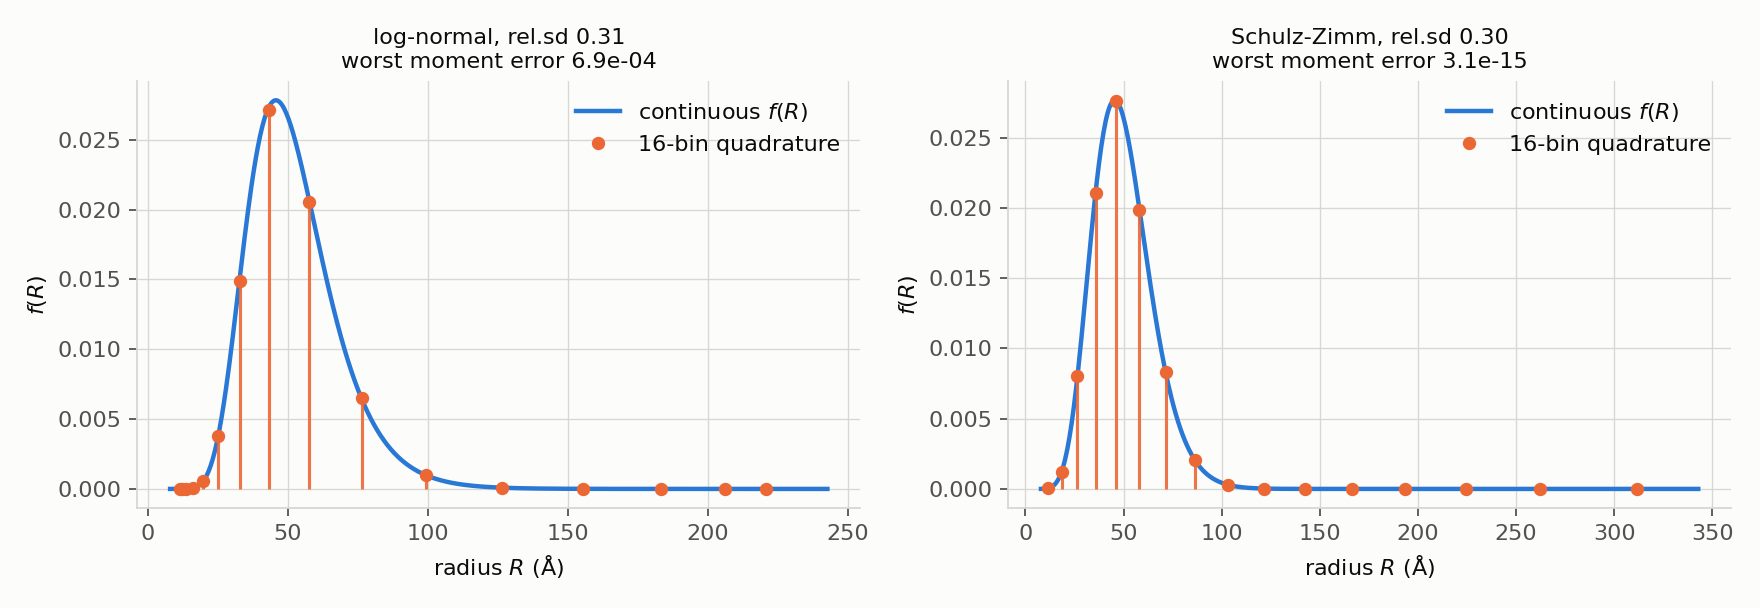
\includegraphics[width=\textwidth]{fig1_distribution.png}
\caption{Continuous size distributions and their quadrature representation.
Schulz--Zimm moments are reproduced to machine precision at any width; the
log-normal to $\sim10^{-4}$ at these settings.}
\label{fig:dist}
\end{figure}

\subsection{Form factors and the intensity}

Two form factors are provided: the homogeneous sphere, and a core--shell
sphere polydisperse in the outer radius (with either a fixed shell thickness
or a fixed core/shell ratio). The hard core and the Yukawa tail act on the
\emph{outer} diameter, so two systems differing only in internal contrast share
identical $S_{ij}(Q)$ --- structure and form factor remain separable, which is
precisely what the decoupling approximation destroys.

The exact intensity is \eqref{eq:Iexact}. Its validation is summarised in
Table~\ref{tab:sasval}; note that in the first two rows the residual scales as
$\mathrm{relsd}^2$ and as $\varphi$ respectively, i.e.\ it is the genuine
physical effect being switched off, not numerical error.

\begin{table}[htbp]
\centering\small
\caption{Validation of the scattering layer.}
\label{tab:sasval}
\begin{tabular}{@{}ll@{}}
\toprule
Check & Result\\
\midrule
monodisperse limit, $\mathrm{relsd}\to0$, vs.\ reference $n|F|^2S(Q)$
  & $3.1\times10^{-5}$ at $10^{-3}$; $3.1\times10^{-7}$ at $10^{-4}$\\
dilute limit, $\varphi\to0$, vs.\ $n\langle F^2\rangle$
  & $4.6\times10^{-4}$ at $\varphi=10^{-4}$; $4.6\times10^{-6}$ at $10^{-6}$\\
core--shell with zero core contrast $\equiv$ plain sphere & $0$ (exactly)\\
$\sum_{ij}\sqrt{x_ix_j}S_{ij}=S_{\text{number}}$ & $8.9\times10^{-16}$\\
\code{nbins} convergence at low/mid $Q$ ($\code{nbins}=20$) & $\sim10^{-10}$\\
\bottomrule
\end{tabular}
\end{table}

\begin{figure}[htbp]
\centering
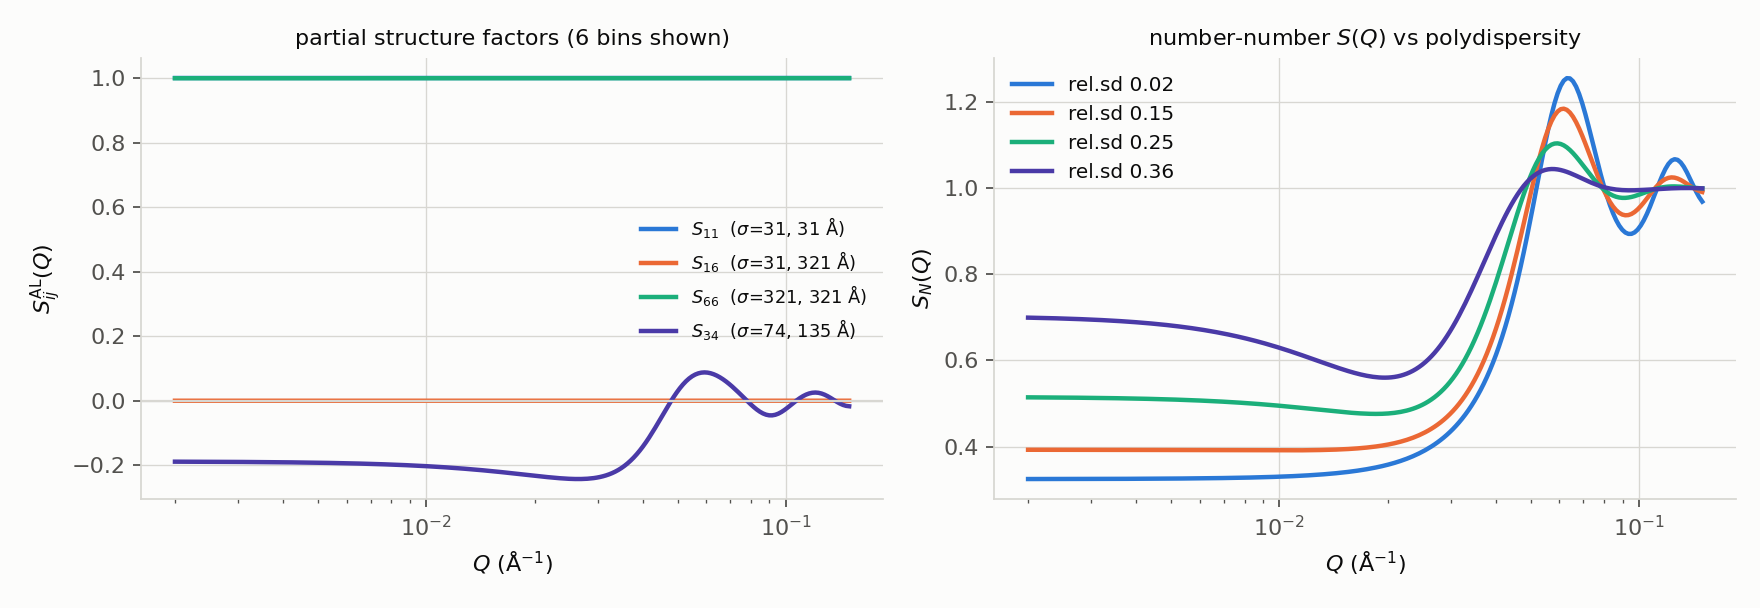
\includegraphics[width=\textwidth]{fig2_partials.png}
\caption{Left: partial structure factors for a six-class discretisation.
Right: the number--number $S(Q)$ as polydispersity increases, at fixed volume
fraction.}
\label{fig:partials}
\end{figure}

\section{Assessment of SASfit's approximations}
\label{sec:approx}

\subsection{The six schemes}

SASfit implements six ways of folding a structure factor into a polydisperse
intensity. They are transcribed here from SASfit's own manual
(\code{doc/manual/SASfit\_ch3.tex}); the GUI exposes the first five as
radio buttons, while the sixth is documented but not offered there. With
$n$ the total number density and $w_i$ the number weights,
\begin{align}
  \text{0 monodisperse:}\quad & I=n\langle F^2\rangle S(Q)\\
  \text{1 decoupling \cite{Kotlarchyk1983}:}\quad
    & I=n\big\{\langle F^2\rangle+\langle F\rangle^2[S(Q)-1]\big\}\\
  \text{2 local monodisperse \cite{Pedersen1994}:}\quad
    & I=n\sum_i w_iF_i^2\,S(Q;R_i)\\
  \text{3 partial structure factors:}\quad
    & I=n\big\{\langle F^2\rangle+\textstyle\sum_{ij}w_iw_jF_iF_j[S_{ij}-1]\big\}\\
  \text{4 scaling \cite{Gazzillo1999}:}\quad
    & \text{as 3, each term}\times\bar V_{ij}/V_{\mathrm{av}}\\
  \text{5 van der Waals one-fluid:}\quad
    & \text{as 4, normalised by }\langle\bar V\rangle
\end{align}
with $\bar V_{ij}=\tfrac{4\pi}{3}\big(\tfrac{R_i+R_j}{2}\big)^3$,
$V_{\mathrm{av}}=\langle V_i\rangle$ and
$\langle\bar V\rangle=\sum_{ij}w_iw_j\bar V_{ij}$.

The essential point about schemes 3--5 is that their ``$S_{ij}$'' is
\emph{not} a true partial structure factor: it is the \emph{monodisperse}
$S(Q)$ evaluated at the mean radius $(R_i+R_j)/2$. That substitution is exactly
what an exact $S_{ij}$ removes, so the comparison below isolates its cost.

\subsection{Method}

Three interactions are used: an attractive Yukawa ($K=+1$), a repulsive Yukawa
($K=-1$; recall the sign convention of \S2.1), and polydisperse adhesive hard
spheres, for which the exact
$S_{ij}$ is taken from SASfit's own Robertus engine
\cite{Robertus1989} --- a completely independent implementation, with no part
of the Blum--Hernando machinery involved. All three run through
\emph{byte-identical} approximation code, so any difference between them is
physics rather than implementation.

Errors are reported as the worst relative deviation from the exact result over
the $Q$ range carrying signal, defined as $I_{\text{exact}}>1\%$ of its low-$Q$
value. A plain maximum over all $Q$ is not usable: $I(Q)$ spans decades and
passes through form-factor minima where it nearly vanishes, so any ratio
explodes there --- and those minima are \emph{deepest at low polydispersity},
producing a spurious error floor exactly where every scheme must become exact.

\subsection{Results}

\begin{table}[htbp]
\centering\small
\caption{Worst error in $I(Q)$ (\%) against the exact result, at
$\varphi=0.20$. Log-normal sizes; $Z=6$ for the Yukawa cases, $\tau=0.2$ for
the adhesive spheres. Best scheme in each row in bold.}
\label{tab:approx}
\begin{tabular}{@{}lrrrrrr@{}}
\toprule
rel.\ s.d. & 0 mono & 1 decoup & 2 LMA & 3 partial & 4 scaling & 5 vdW1\\
\midrule
\multicolumn{7}{@{}l}{\itshape attractive Yukawa, $K=+1$}\\
$0.03$ & $1.3$ & $1.8$ & $1.0$ & $1.8$ & $0.3$ & $\bm{0.2}$\\
$0.10$ & $11.1$ & $19.9$ & $5.2$ & $19.4$ & $3.5$ & $\bm{2.6}$\\
$0.20$ & $16.9$ & $71.0$ & $\bm{5.3}$ & $69.6$ & $12.2$ & $9.5$\\
$0.31$ & $28.8$ & $125.2$ & $\bm{9.0}$ & $123.5$ & $20.7$ & $19.3$\\
\midrule
\multicolumn{7}{@{}l}{\itshape repulsive Yukawa, $K=-1$}\\
$0.03$ & $0.9$ & $3.6$ & $0.8$ & $3.6$ & $\bm{0.2}$ & $0.8$\\
$0.10$ & $9.4$ & $35.2$ & $7.5$ & $35.5$ & $\bm{1.6}$ & $7.9$\\
$0.20$ & $25.1$ & $98.8$ & $21.9$ & $99.7$ & $\bm{4.8}$ & $23.4$\\
$0.31$ & $39.2$ & $141.5$ & $33.3$ & $142.5$ & $\bm{7.2}$ & $39.0$\\
\midrule
\multicolumn{7}{@{}l}{\itshape adhesive hard spheres, $\tau=0.2$ (Robertus)}\\
$0.03$ & $0.7$ & $0.4$ & $1.0$ & $0.4$ & $\bm{0.1}$ & $\bm{0.1}$\\
$0.10$ & $7.3$ & $4.7$ & $5.6$ & $4.4$ & $\bm{1.0}$ & $1.5$\\
$0.20$ & $19.3$ & $16.4$ & $\bm{4.2}$ & $15.0$ & $4.0$ & $5.5$\\
$0.31$ & $26.8$ & $29.4$ & $\bm{7.5}$ & $27.0$ & $8.8$ & $11.4$\\
\bottomrule
\end{tabular}
\end{table}

\begin{figure}[htbp]
\centering
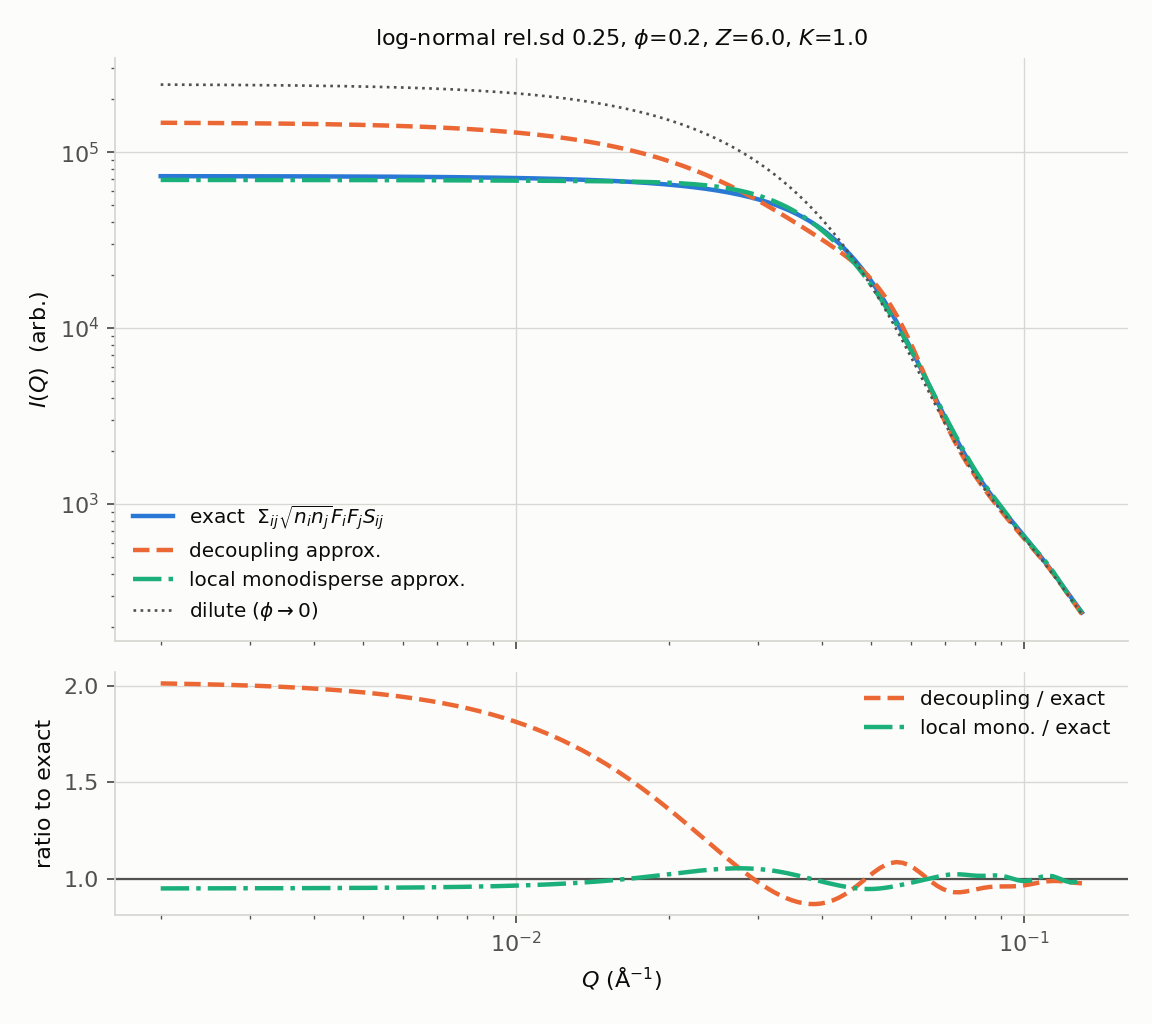
\includegraphics[width=\textwidth]{fig3_intensity.png}
\caption{Exact $I(Q)$ against the decoupling and local monodisperse
approximations, log-normal sizes with rel.\ s.d.\ $0.25$ at $\varphi=0.20$.
Lower panel: ratio to the exact result. Decoupling overestimates $I(Q\to0)$ by
a factor $2.0$.}
\label{fig:intensity}
\end{figure}

\begin{figure}[htbp]
\centering
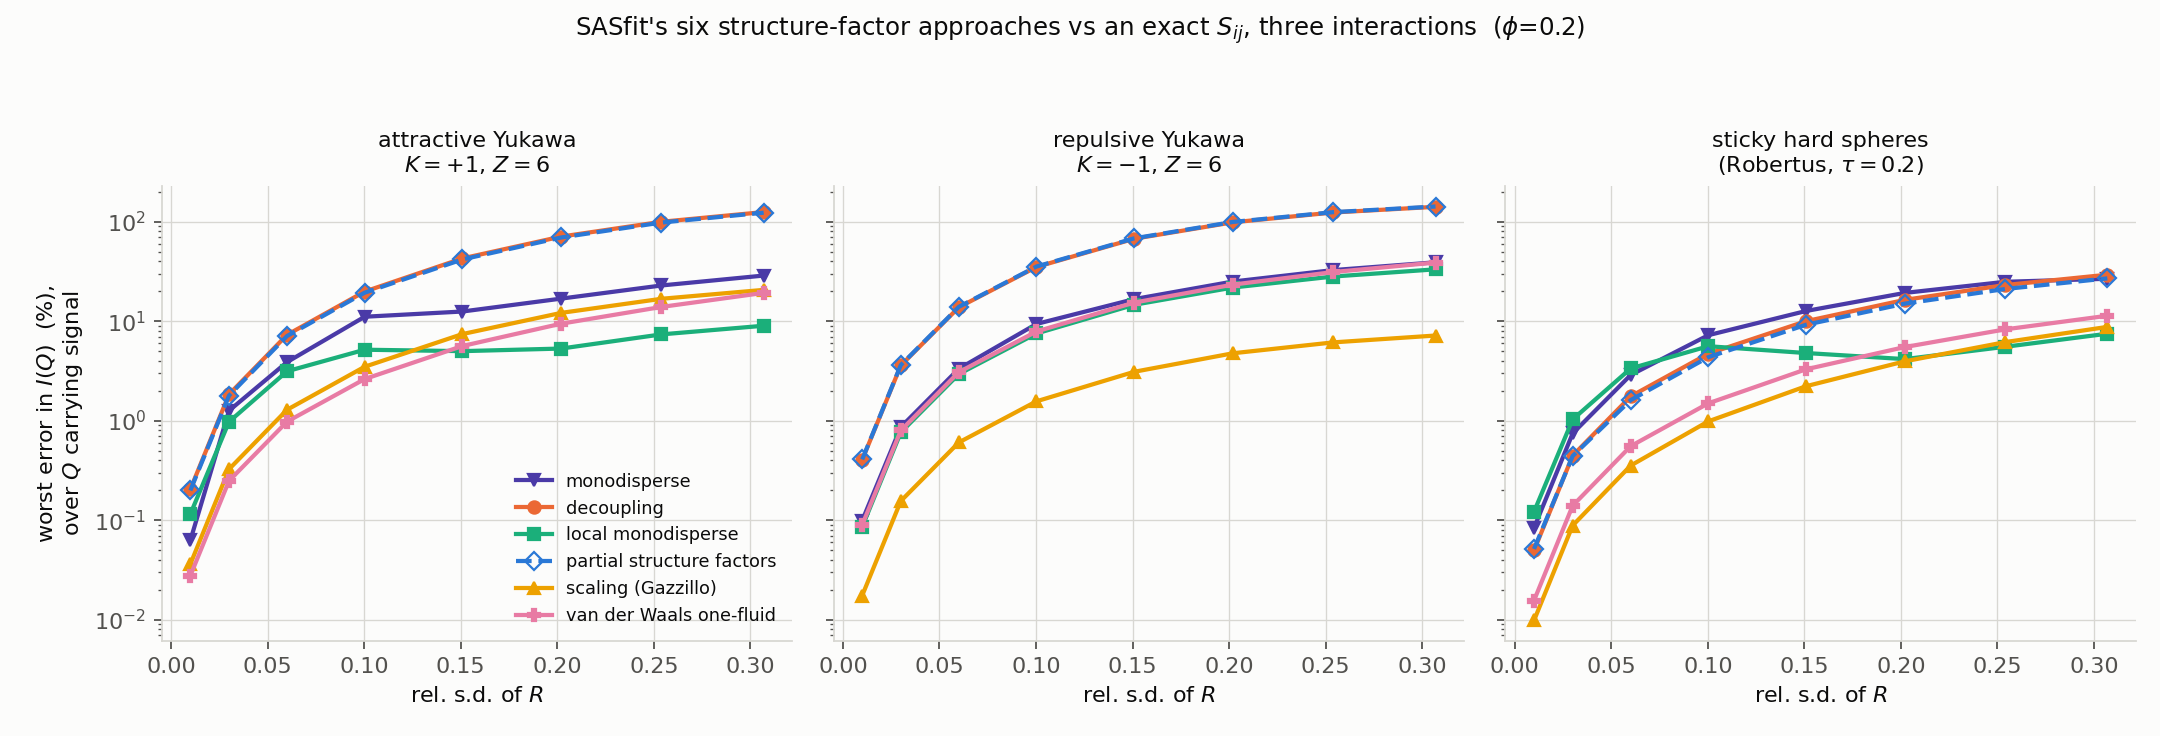
\includegraphics[width=\textwidth]{fig5_three_interactions.png}
\caption{All six schemes against an exact $S_{ij}$, for three interactions.
The ``partial structure factors'' curve (open diamonds, dashed) lies on top of
the decoupling curve throughout. Note that the best-performing scheme changes
between the left and centre panels.}
\label{fig:three}
\end{figure}

\subsection{Discussion}
\label{sec:discussion}

Three conclusions follow from Table~\ref{tab:approx} and
Figure~\ref{fig:three}.

\paragraph{``Partial structure factors'' is indistinguishable from decoupling.}
The two curves coincide at every polydispersity, in all three interactions.
This is structural rather than accidental: scheme 3 substitutes the
monodisperse $S$ at the mean radius, discarding exactly what distinguishes a
true $S_{ij}$, and so inherits decoupling's failure mode intact. Since scheme 3
requires a double integral and scheme 1 does not, scheme 3 is strictly the more
expensive way to obtain the same answer. This appears not to have been
documented before.

\paragraph{The volume weighting is what does the work.} Schemes 4 and 5 differ
from scheme 3 \emph{only} by the factor $\bar V_{ij}/V_{\mathrm{av}}$ (or
$/\langle\bar V\rangle$), and that single factor takes the error from
$\sim125\%$ to $\sim20\%$ for the repulsive Yukawa. Gazzillo's scaling argument
is carrying real physical content.

\paragraph{The ranking depends on the interaction.} For the \emph{attractive}
Yukawa the local monodisperse approximation is best ($9\%$ at rel.\ s.d.\
$0.31$) and scaling is more than twice as bad ($20.7\%$). Reversing the sign of
$K$ reverses the order: for the \emph{repulsive} Yukawa, scaling becomes best by
a wide margin ($7.2\%$) while local monodisperse degrades to $33.3\%$. For
adhesive spheres --- an attractive interaction --- the two are comparable, with
scaling ahead at strong stickiness, consistent with the attractive Yukawa
result.

This matters for practice because the commonest strongly interacting SANS
system, a charge-stabilised colloid, is \emph{repulsive}. The widely used
guidance favouring the local monodisperse approximation is well founded for
attractive systems, but for repulsive ones the scaling approximation of
Gazzillo \emph{et al.} is better by roughly a factor of four. This is a
concrete, testable recommendation that was not previously checkable.

\paragraph{A structural caveat on the local monodisperse approximation.} It can
be \emph{undefined} rather than merely inaccurate. It requires an auxiliary
monodisperse solution at every class diameter, and the small-$\sigma$ classes
correspond to weak screening ($z\sigma_i\sim1$) at the full volume fraction,
where the one-Yukawa MSA has no physical root --- even though the actual
polydisperse system is perfectly well posed. Schemes 3--5 hit the same wall for
the smallest \emph{pairs}. The implementation reports the affected statistical
weight and raises an exception rather than silently returning a curve computed
from a subset of classes.


\section{Extension to the rescaled MSA (RMSA)}
\label{sec:rmsa}

The MSA returns $g_{ij}(\sigma^+_{ij})<0$ for strongly repulsive systems at low
volume fraction --- exactly the charge-stabilised colloids of interest in most
SANS practice. The standard remedy is the rescaled MSA of Hansen and Hayter
\cite{HansenHayter1982}: inflate the hard core, $\sigma\to\lambda\sigma$ with
$\lambda>1$, and fix $\lambda$ by demanding that the rescaled system have
$g(\text{contact})=0$ exactly.

RMSA is therefore \emph{not} a different closure. It is the same MSA applied to
a rescaled system, so the question is only whether the multicomponent solution
admits the rescaling.

\subsection{The rescaling maps onto $\delta_i\neq1$}

The physical potential is fixed; only the reference diameter in
\eqref{eq:closure} changes. Holding $c_{ij}(r)$ fixed while re-referencing
$\sigma_{ij}\to\lambda\sigma_{ij}$ gives
$K'_{ij}=K_{ij}e^{-z(\lambda-1)\sigma_{ij}}$, and because
$\sigma_{ij}=\tfrac12(\sigma_i+\sigma_j)$ this \emph{factorises}:
\begin{equation}
  K'_{ij}=K\,\delta'_i\delta'_j,\qquad
  \boxed{\;\delta'_i=\exp\!\big[-\tfrac{z}{2}(\lambda-1)\sigma_i\big]\;}
  \label{eq:rmsadelta}
\end{equation}
verified to reproduce $c_{ij}(r)$ to $5\times10^{-16}$. Two consequences follow.

\emph{Monodisperse:} $\delta'$ is the same for every species, so it absorbs into
the coupling, $K'=Ke^{-z(\lambda-1)\sigma}$, and the existing $\delta_i=1$
machinery suffices. This is why Hansen--Hayter works as it does.
Table~\ref{tab:rmsa} shows RMSA implemented directly on top of the present
solver: the rescaling drives $g(\sigma'^+)$ to zero to $\sim10^{-13}$ or
better, with physically sensible $\lambda$ between $1.03$ and $1.30$.

\emph{Polydisperse:} $\delta'_i$ depends on $\sigma_i$ and cannot be absorbed.
Polydisperse RMSA is therefore \emph{exactly} the $\delta_i\neq1$ case of
\S\ref{sec:open}, item 1 --- not a separate development.

\begin{table}[htbp]
\centering\small
\caption{Monodisperse RMSA built on the present solver. $g_{\mathrm{MSA}}$ is
the unrescaled contact value; $\lambda$ is the rescaling factor found by
requiring $g=0$ in the rescaled system. Script: \code{rmsa\_extension.py}.}
\label{tab:rmsa}
\begin{tabular}{@{}rrrrrrr@{}}
\toprule
$\varphi$ & $Z$ & $K$ & $g_{\mathrm{MSA}}$ & $\lambda$ & $\varphi_{\mathrm{resc}}$ & $g_{\mathrm{resc}}$\\
\midrule
$0.02$ & $2.0$ & $-1.5$ & $-0.2427$ & $1.0639$ & $0.0241$ & $5\times10^{-17}$\\
$0.02$ & $2.0$ & $-3.0$ & $-1.4081$ & $1.2673$ & $0.0407$ & $-3\times10^{-13}$\\
$0.05$ & $2.0$ & $-3.0$ & $-0.8372$ & $1.1501$ & $0.0761$ & $-2\times10^{-16}$\\
$0.10$ & $2.0$ & $-3.0$ & $-0.1765$ & $1.0285$ & $0.1088$ & $8\times10^{-13}$\\
$0.02$ & $1.0$ & $-3.0$ & $-1.0550$ & $1.2997$ & $0.0439$ & $-6\times10^{-16}$\\
$0.05$ & $1.0$ & $-3.0$ & $-0.4274$ & $1.1087$ & $0.0682$ & $-3\times10^{-15}$\\
\bottomrule
\end{tabular}
\end{table}

\subsection{Polydisperse RMSA is therefore analytic}

Since \S\ref{sec:delta} supplies $\delta_i\neq1$ in closed form, the rescaled
system can be solved directly and no numerical fallback is needed. We adopt a
\emph{common} rescaling factor for all species --- a size-dependent
$\lambda_i$ would destroy the factorisation \eqref{eq:rmsadelta} and with it
the analytic solution --- and fix it by requiring every contact value to be
non-negative, i.e.\ that the binding pair just reach zero:
\begin{equation}
  \min_{ij}\;g_{ij}(\lambda\sigma_{ij})=0 .
  \label{eq:rmsacond}
\end{equation}
The number densities are physical and unchanged, so
$\varphi\to\lambda^3\varphi$ follows automatically.

Table~\ref{tab:rmsapoly} shows the result. The condition is met to
$\sim10^{-14}$, every $g_{ij}$ is then non-negative, and $\lambda=1$ is
returned unchanged when the plain MSA is already physical.

\begin{table}[htbp]
\centering\small
\caption{Polydisperse RMSA with a common $\lambda$ fixed by
\eqref{eq:rmsacond}. Number fractions $0.6:0.4$ for $N=2$ and
$0.5:0.35:0.15$ for $N=3$. Script: \code{polydisperse\_rmsa.py}.}
\label{tab:rmsapoly}
\begin{tabular}{@{}llrrrrr@{}}
\toprule
$\sigma$ & $\varphi$ & $Z$ & $K$ & $\min g_{ij}$ (MSA) & $\lambda$ & $\varphi_{\mathrm{resc}}$\\
\midrule
$[1,1.6]$ & $0.02$ & $2$ & $-3$ & $-1.6635$ & $1.3110$ & $0.0451$\\
$[1,1.6]$ & $0.05$ & $2$ & $-3$ & $-1.2733$ & $1.2242$ & $0.0917$\\
$[1,1.6]$ & $0.10$ & $2$ & $-3$ & $-0.7658$ & $1.1212$ & $0.1409$\\
$[1,1.4,2]$ & $0.05$ & $2$ & $-3$ & $-1.3478$ & $1.2365$ & $0.0945$\\
$[1,1.6]$ & $0.05$ & $1$ & $-3$ & $-0.9367$ & $1.2398$ & $0.0953$\\
$[1,1.6]$ & $0.05$ & $2$ & $-0.5$ & $+0.6768$ & $1$ (none needed) & $0.0500$\\
\bottomrule
\end{tabular}
\end{table}

\paragraph{Cross-validation.} For $\sigma=[1,1.6]$, $\varphi=0.05$, $Z=2$,
$K=-3$ the analytic route gives $\lambda=1.224213$ and the independent
numerical OZ solver, which shares no equation with it, gives $1.224143$ --- a
difference of $0.006\%$.

\paragraph{The small particles set the rescaling.} In every case tested the
binding pair is the smallest--smallest one. This follows directly from
\eqref{eq:rmsadelta}: $\delta'_i=e^{-z(\lambda-1)\sigma_i/2}$ is largest for
the smallest $\sigma_i$, so $K'_{11}$ is the strongest repulsion and $g_{11}$
is the first contact value to go negative. The consequence is that a small
minority population can force a substantial inflation of \emph{every} diameter.

\subsection{An unresolved question of principle}

Condition \eqref{eq:rmsacond} is a choice, not a derivation, and it is worth
being explicit about what it costs. Monodisperse RMSA has one contact value
and one rescaling parameter, so $g(\sigma'^+)=0$ determines $\lambda$ uniquely.
A mixture has $N(N{+}1)/2$ contact values and still only one $\lambda$, and
they do not reach zero together: for the second row of
Table~\ref{tab:rmsapoly}, $g_{11}$ vanishes at $\lambda=1.2242$ while at that
same $\lambda$ the others sit at $g_{12}=0.529$ and $g_{22}=0.845$. Requiring
the minimum to vanish repairs the worst-behaved pair and leaves the rest
strictly positive --- over-corrected relative to their own thresholds.

The alternatives each have a cost: a composition-weighted condition would
leave some $g_{ij}$ negative, defeating the purpose; species-dependent
$\lambda_i$ would break the factorisation \eqref{eq:rmsadelta}, and with it the
analytic solution, forcing the numerical route. We are not aware of a settled
answer in the literature. It should be treated as a modelling decision made
deliberately, not inherited from whichever convention an implementation
happens to adopt.

\section{Limitations and open items}
\label{sec:open}

\begin{enumerate}\itemsep2pt
\item \textbf{Charge polydispersity and polydisperse RMSA} ---
  \emph{resolved}, see \S\ref{sec:delta} and \S\ref{sec:rmsa}. Both follow in
  closed form once \eqBH{22} is corrected. Listed here because earlier drafts
  of this work recorded them as the principal open item; the remaining
  uncertainty is the choice of rescaling condition
  \eqref{eq:rmsacond}, which is a modelling decision rather than a gap in the
  theory.
\item \textbf{Multiple Yukawa terms ($M>1$).} Only $M=1$ is implemented. The
  $M(M-1)$ symmetry conditions of BH02 \S4 become active for $M>1$; the
  $\Gamma$-centric formulation of \eqref{eq:gammaclosure} was written with that
  generalisation in mind.
\item \textbf{Complex $z_n$.} Oscillatory closures are not supported.
\item \textbf{Very broad distributions} --- \emph{this item was wrong, and is
  withdrawn.} Earlier drafts recorded that above rel.\ s.d.\ $\approx0.4$ the
  quadrature could not simultaneously preserve $\langle R^6\rangle$ and keep
  $z\sigma_{\max}$ small enough for the $S_{ij}$ assembly. That was inferred
  from the wrong diagnostic. A Gauss--Laguerre grid places its outermost nodes
  at enormous radii carrying no weight whatever --- at rel.\ s.d.\ $0.5$ and
  $N=96$ the largest node sits at $z\sigma=548$ with $w=5\times10^{-151}$, a
  species containing no particles --- so $z\sigma_{\max}$ taken over all bins
  says nothing about the calculation's health. The span over bins that
  actually hold particles is $0.2$--$17$ and is essentially independent of
  $N$. Measured over $N=12$ to $200$, at nominal $z\sigma_{\max}$ up to $548$:
  the contact-matrix symmetry, the \eqBH{72} residual and the $S_{ij}$ sum
  rule all remain at $10^{-15}$, and $I(Q)$ converges cleanly
  ($1.5\times10^{-3}$ at $N=12$, $1.2\times10^{-9}$ at $N=24$,
  $9\times10^{-14}$ at $N=48$ for rel.\ s.d.\ $0.2$; $6\times10^{-1}$,
  $8.7\times10^{-2}$, $1.9\times10^{-4}$ for rel.\ s.d.\ $0.5$). Broad
  distributions are therefore not out of reach --- they simply need more bins,
  and more bins work. $N=200$ costs about $5$~s. The guard now tests the
  weight-bearing span.
\item \textbf{Unphysical MSA solutions.} At strong attraction the MSA can
  return $g_{ij}(\sigma^+)<0$. This is a property of the closure, not of the
  implementation, but callers should test for it.
\item \textbf{Size-independent stickiness.} The Robertus comparison inherits
  that engine's assumption $\tau_{nm}=\tau$, so its polydispersity is purely in
  size --- the same restriction as $\delta_i=1$ on the Yukawa side.
\end{enumerate}

\section{Software}

\begin{longtable}{@{}ll@{}}
\toprule
File & Role\\
\midrule
\endhead
\code{polydisperse\_yukawa\_msa.py} & closure solver; \code{solve()} and \code{solve\_gamma()}; contact values\\
\code{polydisperse\_yukawa\_sq.py} & $S_{ij}(Q)$ assembly, \eqref{eq:SQ}\\
\code{polydisperse\_sas\_base.py} & exact $I(Q)$ and all six approximations (shared)\\
\code{polydisperse\_yukawa\_sas.py} & size distributions, form factors, Yukawa model\\
\code{robertus\_shs\_sas.py} & adhesive-sphere model on the same base\\
\code{robertusWrapper.py} & ctypes wrapper for SASfit's \code{robertus\_shs\_core.c}\\
\code{polydisperse\_rmsa.py} & polydisperse RMSA, common $\lambda$, condition \eqref{eq:rmsacond}\\
\code{mixture\_oz\_numerical.py} & independent numerical multicomponent OZ solver\\
\midrule
\code{sas\_validation.py} & scattering-layer validation\\
\code{gamma\_solve\_validation.py} & the six $N>1$ conditions\\
\code{external\_N\_validation.py} & numerical vs.\ corrected vs.\ as-printed\\
\code{PiX\_two\_routes.py} & \eqBH{34}/\eqBH{37} against \eqBH{30}/\eqBH{32}/\eqBH{33}\\
\code{Jhat\_derivation\_check.py} & derived vs.\ printed $\hat{\mathcal J}$; the three $P^{(n)}$\\
\code{eq100\_gamma\_check.py} & \eqBH{100}/\eqBH{100b} independent contact route\\
\code{blum\_arias\_IJ\_check.py} & adjudicates \eqBH{35}/\eqBH{38} against BA \eqBH{76} (Table~\ref{tab:adjudication})\\
\code{eq22\_symmetry\_test.py} & decides the \eqBH{22} index by $g_{ij}=g_{ji}$ alone (Table~\ref{tab:symmetry})\\
\code{delta\_general.py} & second route to general $\delta_i$, via \eqBH{51}--\eqBH{53}\\
\code{contact\_exact\_verify.py} & contact value vs.\ the compiled library and the Lebowitz mixture limit\\
\code{rmsa\_extension.py} & the rescaling algebra and monodisperse RMSA\\
\code{report\_numbers.py} & regenerates every number in this report\\
\bottomrule
\end{longtable}

\paragraph{Building the Robertus engine off Windows.} It requires GSL and
SUNDIALS $\ge6$. The source targets SUNDIALS 7.x; on 6.x a small
error-handler shim added with \code{-include} suffices, leaving the SASfit
source itself unmodified:
\begin{verbatim}
gcc -O2 -fPIC -shared -include rshs/sundials6_shim.h -o librobertus.so \
    robertus_shs_core.c -lgsl -lgslcblas -lsundials_kinsol \
    -lsundials_nvecserial -lm
\end{verbatim}
On Windows the wrapper locates SASfit's prebuilt
\code{libsasfit\_robertus\_shs.dll} automatically, or honours the
\code{ROBERTUS\_SHS\_LIB} environment variable.

\begin{thebibliography}{9}
\bibitem{Blum2002} L.~Blum and J.~A.~Hernando,
  \emph{Yukawa fluids in the mean spherical approximation: I. The general
  solution}, J.~Phys.: Condens.\ Matter \textbf{14}, 11933 (2002).
\bibitem{BlumArias} L.~Blum and M.~Arias,
  \emph{Structure of multi-component/multi-Yukawa mixtures},
  arXiv:cond-mat/0602477 (2006).
\bibitem{HoyeBlum1977} J.~S.~Høye and L.~Blum,
  \emph{Solution of the Yukawa closure of the Ornstein--Zernike equation},
  J.~Stat.\ Phys.\ \textbf{16}, 399 (1977).
\bibitem{BlumHoye1978} L.~Blum and J.~S.~Høye,
  \emph{Solution of the Ornstein--Zernike equation with Yukawa closure for a
  mixture}, J.~Stat.\ Phys.\ \textbf{19}, 317 (1978).
\bibitem{Blum1980} L.~Blum,
  \emph{Solution of the Ornstein--Zernike equation for a mixture of hard ions
  and Yukawa closure}, J.~Stat.\ Phys.\ \textbf{22}, 661 (1980).
\bibitem{Niizeki1981} K.~Niizeki,
  \emph{Solution of the Ornstein--Zernike equation for a multicomponent system
  with Yukawa closure}, Mol.\ Phys.\ \textbf{43}, 251 (1981).
\bibitem{GinozaYasutomi1997} M.~Ginoza and M.~Yasutomi,
  \emph{An extension of the analytical solution of the Ornstein--Zernike
  equation with the Yukawa closure},
  J.~Stat.\ Phys.\ \textbf{90}, 1475 (1998).
\bibitem{GinozaYasutomi1998} M.~Ginoza and M.~Yasutomi,
  \emph{Analytical model for thermodynamic properties of a colloidal dispersion
  with size and `charge' polydispersities},
  Mol.\ Phys.\ \textbf{95}, 163 (1998).
\bibitem{Kalyuzhnyi2006} Yu.~V.~Kalyuzhnyi and S.~P.~Hlushak,
  \emph{Phase coexistence in polydisperse multi-Yukawa hard-sphere fluid: high
  temperature approximation}, J.~Chem.\ Phys.\ \textbf{125}, 034501 (2006).
\bibitem{Baxter1968} R.~J.~Baxter,
  \emph{Percus--Yevick equation for hard spheres with surface adhesion},
  J.~Chem.\ Phys.\ \textbf{49}, 2770 (1968).
\bibitem{Wertheim1963} M.~S.~Wertheim,
  \emph{Exact solution of the Percus--Yevick integral equation for hard
  spheres}, Phys.\ Rev.\ Lett.\ \textbf{10}, 321 (1963).
\bibitem{Kotlarchyk1983} M.~Kotlarchyk and S.-H.~Chen,
  \emph{Analysis of small angle neutron scattering spectra from polydisperse
  interacting colloids}, J.~Chem.\ Phys.\ \textbf{79}, 2461 (1983).
\bibitem{Pedersen1994} J.~S.~Pedersen,
  \emph{Determination of size distributions from small-angle scattering data
  for systems with effective hard-sphere interactions},
  J.~Appl.\ Cryst.\ \textbf{27}, 595 (1994).
\bibitem{Gazzillo1999} D.~Gazzillo, A.~Giacometti, R.~G.~Della Valle,
  E.~Venuti and F.~Carsughi,
  \emph{A scaling approximation for structure factors in the integral equation
  theory of polydisperse nonionic colloidal fluids},
  J.~Chem.\ Phys.\ \textbf{111}, 7636 (1999).
\bibitem{HansenHayter1982} J.-P.~Hansen and J.~B.~Hayter,
  \emph{A rescaled MSA structure factor for dilute charged colloidal
  dispersions}, Mol.\ Phys.\ \textbf{46}, 651 (1982).
\bibitem{Robertus1989} C.~Robertus, W.~H.~Philipse, J.~G.~H.~Joosten and
  Y.~K.~Levine, \emph{Solution of the Percus--Yevick approximation of the
  multicomponent adhesive spheres system applied to the small angle x-ray
  scattering from a water-in-oil microemulsion},
  J.~Chem.\ Phys.\ \textbf{90}, 4482 (1989).
\end{thebibliography}

\end{document}
